% This is the University of Chicago Graham School Master of Science in Analytics
% template. Much of it is based on the Reed College LaTeX thesis template.
% Most of the work for the Reec College template was done by Sam Noble (SN),
% Later comments etc. by Ben Salzberg (BTS).
% Additional restructuring and APA support by Jess Youngberg (JY).
% Justin M. Shea (JMS) built on their good open source work.
% Your comments and suggestions are more than welcome:
% please email, them to justinshea@uchicago.edu.
%
% Any line that starts with a percent symbol is a comment.
% They won't show up in the document, and are useful for notes
% to yourself and explaining commands.
% Commenting also removes a line from the document;
% very handy for troubleshooting problems. -BTS
%%
%% Preamble
%%
% \documentclass{<something>} must begin each LaTeX document
% Added by JMS
\documentclass[12pt,oneside]{chicagocapstone}
% END of JMS add
% Packages are extensions to the basic LaTeX functions. Whatever you
% want to typeset, there is probably a package out there for it.
% Check out CTAN to see: http://www.ctan.org/
%%
\usepackage{graphicx,latexsym}
\usepackage{amsmath}
\usepackage{amssymb,amsthm}
\usepackage{longtable,booktabs,setspace}
\usepackage[hyphens]{url}
% Added by CII
\usepackage{hyperref}
\usepackage{lmodern}
\usepackage{float}
\floatplacement{figure}{H}
% End of CII addition
\usepackage{rotating}


% Added by CII (Thanks, Hadley!)
% Use ref for internal links
\renewcommand{\hyperref}[2][???]{\autoref{#1}}
\def\chapterautorefname{Chapter}
\def\sectionautorefname{Section}
\def\subsectionautorefname{Subsection}
% End of CII addition

% Added by CII
\usepackage{caption}
\captionsetup{width=5in}
% End of CII addition

% Added by JMS
\usepackage{mathptmx} % Times New Roman fonts
% End of add by JMS

% Syntax highlighting #22

% To pass between YAML and LaTeX the dollar signs are added by CII
\title{Data Analytics as a Service (DAaaS): Automated \& Intelligent Imputation
Methods for Supervised Machine Learning}
\author{Shahid Barkat, Joseph Kearney}
\date{June, 2019} % The month and year that you submit your FINAL draft)
\division{Graham School}
\advisor{Dr.~Arnab Bose}
\institution{University of Chicago}
\degree{Master of Science in Analytics}
\altadvisor{Dr.~Sema Barlas}
% End of CII addition

\department{Continuing Liberal and Professional Studies}

% Added by CII
%%% Copied from knitr
%% maxwidth is the original width if it's less than linewidth
%% otherwise use linewidth (to make sure the graphics do not exceed the margin)
\makeatletter
\def\maxwidth{ %
  \ifdim\Gin@nat@width>\linewidth
    \linewidth
  \else
    \Gin@nat@width
  \fi
}
\makeatother

\renewcommand{\contentsname}{Table of Contents}
% End of CII addition

\setlength{\parskip}{0pt}

% Added by CII
  %\setlength{\parskip}{\baselineskip}
  \usepackage[parfill]{parskip}

\providecommand{\tightlist}{%
  \setlength{\itemsep}{0pt}\setlength{\parskip}{0pt}}


\Abstract{
The researchers develop and maintain an open-source, Python-based
package named Autoimpute to address one of the most common nuisances in
machine learning -- datasets with missing values. The package implements
numerous imputation algorithms and extends common supervised machine
learning methods to handle multiply imputed datasets. Autoimpute treats
missing data as a first-class citizen in the Python world, making
imputation familiar to Python developers and easy to use for those new
to the language. Ultimately, the package provides users an end-to-end
framework that covers missing data exploration to imputation analysis.

\bigskip  \bigskip
\bigskip

\textbf{Keywords}: Missing Data; Imputation; Python; Autoimpute Package;
Machine Learning; Bias/Variance Analysis; Fractional Factorial Design,
SciKit Learn; Pandas
}

% Added by JMS
\Executive{
This research develops an end-to-end methodology to address one of the
most common nuisances in machine learning -- datasets with missing
values. It approaches incomplete datasets with four objectives: describe
and visualize the extent of the missing value problem; examine factors
related to missingness; develop methods to impute missing data; and
measure the impact of imputation on inference derived from supervised
learning, specifically linear and logistic regression.

To meet these objectives, the researchers develop and maintain an
open-source, Python-based package named Autoimpute. The package works
with pandas DataFrames and implements numerous imputation algorithms,
which the authors cover later in this report. Autoimpute also extends
common supervised machine learning methods to handle imputed datasets.
The package includes linear and logistic regression specifically
designed for multiply imputed data as well as methods to assess the
impact of imputation on parameter inference from these analysis models.
Further, Autoimpute follows the API design of popular Python machine
learning package, scikit-learn. Its ``Imputers'' integrate nicely with
scikit-learn machine learning pipelines.

Autoimpute treats missing data as a first-class citizen in the Python
world, making imputation familiar to Python developers and easy to use
for those new to the language. The package incorporates the four
objectives outlined above and provides users an end-to-end framework
that covers missing data exploration to imputation analysis. In doing
so, Autoimpute remains flexible, yielding users as much control and
complexity as they would like while they grapple with missing data.
}
% End of JMS add

\Acknowledgements{

}

\Dedication{

}

\Preface{

}


	\usepackage{array} \usepackage{multirow} \usepackage{booktabs}
\usepackage{colortbl} \usepackage{makecell} \usepackage{xcolor}
\usepackage{tabu} \usepackage{amsmath}
% End of CII addition
%%
%% End Preamble
%%
%
\begin{document}

% Everything below added by CII
  \maketitle

\frontmatter % this stuff will be roman-numbered
\pagestyle{empty} % this removes page numbers from the frontmatter


%% Reorganized by JMS
  \begin{abstract}
    The researchers develop and maintain an open-source, Python-based
    package named Autoimpute to address one of the most common nuisances in
    machine learning -- datasets with missing values. The package implements
    numerous imputation algorithms and extends common supervised machine
    learning methods to handle multiply imputed datasets. Autoimpute treats
    missing data as a first-class citizen in the Python world, making
    imputation familiar to Python developers and easy to use for those new
    to the language. Ultimately, the package provides users an end-to-end
    framework that covers missing data exploration to imputation analysis.
    
    \bigskip  \bigskip
    \bigskip
    
    \textbf{Keywords}: Missing Data; Imputation; Python; Autoimpute Package;
    Machine Learning; Bias/Variance Analysis; Fractional Factorial Design,
    SciKit Learn; Pandas
  \end{abstract}
 % Added by JMS
  \begin{executive}
    This research develops an end-to-end methodology to address one of the
    most common nuisances in machine learning -- datasets with missing
    values. It approaches incomplete datasets with four objectives: describe
    and visualize the extent of the missing value problem; examine factors
    related to missingness; develop methods to impute missing data; and
    measure the impact of imputation on inference derived from supervised
    learning, specifically linear and logistic regression.
    
    To meet these objectives, the researchers develop and maintain an
    open-source, Python-based package named Autoimpute. The package works
    with pandas DataFrames and implements numerous imputation algorithms,
    which the authors cover later in this report. Autoimpute also extends
    common supervised machine learning methods to handle imputed datasets.
    The package includes linear and logistic regression specifically
    designed for multiply imputed data as well as methods to assess the
    impact of imputation on parameter inference from these analysis models.
    Further, Autoimpute follows the API design of popular Python machine
    learning package, scikit-learn. Its ``Imputers'' integrate nicely with
    scikit-learn machine learning pipelines.
    
    Autoimpute treats missing data as a first-class citizen in the Python
    world, making imputation familiar to Python developers and easy to use
    for those new to the language. The package incorporates the four
    objectives outlined above and provides users an end-to-end framework
    that covers missing data exploration to imputation analysis. In doing
    so, Autoimpute remains flexible, yielding users as much control and
    complexity as they would like while they grapple with missing data.
  \end{executive}
 % End of JMS




  \hypersetup{linkcolor=black}
  \setcounter{tocdepth}{2}
  \tableofcontents

  \listoffigures

  \listoftables

%% END of Reorganization by JMS

\mainmatter % here the regular arabic numbering starts
\pagestyle{fancyplain} % turns page numbering back on

\chapter*{Introduction}\label{introduction}
\addcontentsline{toc}{chapter}{Introduction}

The researchers develop and maintain an open-source, Python-based
package named \texttt{Autoimpute} to address one of the most common
nuisances in machine learning -- datasets with missing values. The
package implements numerous imputation algorithms and extends common
supervised machine learning methods to handle multiply imputed datasets.
\texttt{Autoimpute} treats missing data as a first-class citizen in the
Python world, making imputation familiar to Python developers and easy
to use for those new to the language. Ultimately, the package provides
users an end-to-end framework that covers missing data exploration to
imputation analysis.

\section*{Problem Statement}\label{problem-statement}
\addcontentsline{toc}{section}{Problem Statement}

Machine learning models rely entirely on the data they are provided, and
most require that the underlying dataset be complete. In reality,
however, many real-world datasets are incomplete, containing missing
values for the response variable and one or more of the features
collected. As a result, the machine learning practitioner must decide
what to do about missing data. The way in which the practitioner handles
missing data greatly affects the interpretability of and results from
the machine learning models the practitioner builds and deploys.

The challenge of handling missing data has inspired numerous imputation
methods, each of which has its advantages and disadvantages depending on
the nature of the missing data and the machine learning task at hand.
Unfortunately, the existence of multiple imputation methods does not get
the machine learning practitioner any closer to handling missing data.
First, imputation methods can be challenging to understand and
computationally expensive to implement. Next, no global criteria or
metric exists to select the optimal imputation method given a dataset
with missing values. Even if a practitioner successfully implements
imputation methods, he or she has no structured way to evaluate how well
imputation performs or how imputation affects supervised models
downstream built upon imputed data.

Because handling missing data is quite complex, most statistical
packages simply remove records with missing data so that machine
learning models can execute. While this option is simple to implement
and enables models to run, it generally comes with numerous undesirable
side effects if data is not missing completely at random (MCAR). This
subject is explored further in the background section of this paper.
However, in practice, real-world data is rarely MCAR, so models should
generally avoid discarding missing records. Extensions in software
packages do exist to implement imputation methods automatically. That
being said, the practitioner still must decide which method to
implement, explain why an imputation method is optimal, and evaluate how
the optimal imputation method affects models trained on imputed data.

\section*{Research Purpose}\label{research-purpose}
\addcontentsline{toc}{section}{Research Purpose}

This research aids the machine learning practitioner by bringing more
clarity to the imputation process, making imputation methods more
accessible and comparable, and measuring the impact imputation methods
have in supervised regression and classification models. This research
strives to not just automate imputation but also develop an open-source
framework to structure and evaluate imputation methods within a
supervised machine learning process.

To address this purpose, this research specifies four objectives:
\begin{enumerate}
\def\labelenumi{\arabic{enumi}.}
\tightlist
\item
  Assess the extent of the missing data problem with descriptive and
  visual measures
\item
  Examine the factors related to the missingness of data
\item
  Deploy imputation methods and select the most appropriate methodology
\item
  Measure the impact of imputation to the fit, stability, bias, and
  variance of parameters derived from supervised models built on imputed
  data
\end{enumerate}
The researchers meet these objectives by developing an open-source
Python package that can generalize across cross-sectional and
time-series datasets. Any data science professional can deploy or reuse
components of the package itself. Eventually, the researchers will
accept contributions from the open source community as well.

\hypertarget{background}{\chapter*{Background}\label{background}}
\addcontentsline{toc}{chapter}{Background}

One must understand what missingness is and why it exists before
deciding how to handle it. The authors explore the nature of missingness
using a motivating example.

For an experiment, assume that a random sample of measurements is
collected from thousands of weigh scales. Also assume each weigh scale
in the experiment may fail to produce measurements for three separate
reasons. First, a scale might run out of batteries, in which case all
measurements from that scale cease for a given period of time. Next, a
scale may fail more frequently for heavier objects or items over a
certain weight threshhold. And finally, a scale may stop reporting
measurements when placed on a soft surface instead of a hard one (van
Buuren, 2018, ch.~1.2).

As a result of these scenarios, the random sample collected likely has
many instances in which weight measurements are unobserved. How
missingness in this sample is handled moving forward will depend on
characteristics of the missing data itself and the process that
generated missingess. The authors devote the rest of this section to
concepts related to the nature of missingness and how it is handled. The
authors refer back to this example to make concepts more concrete.

\section*{Basic Terminology and Notation}\label{background-basic-terms}
\addcontentsline{toc}{section}{Basic Terminology and Notation}

Before diving into concepts related to missingness, the authors
establish notation used throughout this text. The authors use this
notation to develop mathematical expressions that explain these concepts
succinctly. This research follows the notation van Buuren uses in the
second edition of his book, Flexible Imputation of Missing Data. For
more information, refer to Appendix B, which collects and summarizes the
notation seen throughout this research. Appendix C contains the
equations and expressions that formalize concepts related to missing
data, while Appendix D contains the definitions for the concepts
themselves.

In the introductory example, weigh scales produce a set of \(n\)
measurements, some of which may be missing weight. \(Y\) denotes the
\(n\) x \(p\) matrix that contains the \(n\) measurements and the \(p\)
variables recorded along with the measurements. The surface of the scale
(hard or soft) is an example of a discrete variable in \(p\), while the
weight measurement itself is a continuous variable in \(p\). We can
retrieve an observation within \(Y\) by specifying the row and column
index corresponding to the observation's cell. To do so, we use the
notation \(y_{ij}\), where \(i\) represents the row and \(j\) represents
the column associated with a scalar \(y\) in matrix \(Y\).

\(Y\) itself represents the hypothetically complete data (van Buuren,
2018, ch.~2.2.3), which is comprised of \(Y_{obs}\) and \(Y_{mis}\).
\(Y_{obs}\) represents each row \(Y_i\) out of \(n\) records that have
known values for each column \(Y_j\) in \(p\). \(Y_{mis}\), on the other
hand, contains records with missing observations across any of the
columns in \(p\). Note that \(Y = (Y_{obs}, Y_{mis})\). The
hypothetically complete data equals the conjoined observed and missing
data matrices.

It is convenient to store whether or not a cell in \(Y\) is missing in a
separate matrix \(R\). Therefore, \(R\) is an \(n\) by \(p\) matrix
where all entries \(r_{ij} \in {0, 1}\). Any observation \(r_{ij}=1\)
corresponds to a known value for \(y_{ij}\). On the contrary, any
observation \(r_{ij}=0\) corresponds to a missing value for \(y_{ij}\).
\(R\) is commonly referred to as the \textbf{missing indicator matrix},
while \(Y\) is the \textbf{complete data matrix} (van Buuren, 2018,
ch.~2.2.3).

\section*{Missing Data Mechanism}\label{background-missing-data-mech}
\addcontentsline{toc}{section}{Missing Data Mechanism}

Each of the three scenarios discussed above causes a given weigh scale
to produce missing data, but the underlying reason for missingness is
quite different in each case. Donald Rubin describes the ways in which
data can be missing (Rubin, 1976). According to Rubin (as cited in van
Buuren, 2018, ch.~1.2), every observation in a dataset has some
probability of being missing. The process that governs these
probabilities is called the \textbf{missing data mechanism} (Rubin, as
cited in van Buuren, 2018, ch.~1.2). The missing data mechanism
generates a statistical relationship between observations and the
probability of missing data (Nakagawa, 2015, p.~83). The \textbf{missing
data model} is the function that formalizes that statistical
relationship (van Buuren, 2018, ch.~2.2.4). These statistical
relationships fall into one of three categories, each of which
represents a different missing data mechanism (Rubin, as cited in van
Buuren, 2018, ch.~1.2).

The general expression for the missing data model is defined as:

\[P(R|Y_{obs}, Y_{mis},\psi)\]

\(\psi\) contains the parameters of the missing data model. This
expression notes that the probability of missingness \(P(R=0)\) within a
dataset depends on the observed data, the missing data, and the missing
data model's parameters (van Buuren, 2018, ch.~2.2.4). From another
lense, this expession states that the missing data model is the
distribution of the missingness indicator conditional on the observed
data, the missing data, and the parameters of the missing data model.

The missing data model is the function that formalizes the statistical
relationship governed by a missing data mechanism. The next section
examines the manifestation of the missing data model under each
mechanism.

\subsection*{MCAR, MAR, and MNAR}\label{background-mcar-mar-mnar}
\addcontentsline{toc}{subsection}{MCAR, MAR, and MNAR}

Rubin popularized names for the three categories that represent the main
missing data mechanisms:
\begin{itemize}
\tightlist
\item
  \textbf{Missing Completely at Random (MCAR)}
\item
  \textbf{Missing at Random (MAR)}
\item
  \textbf{Missing Not at Random (MNAR)}
\end{itemize}
In this research, the authors refer to each category by its abbreviated
label. The subsections below examine each category in more detail.

\subsubsection*{Missing Completely at Random (MCAR)}\label{mcar}
\addcontentsline{toc}{subsubsection}{Missing Completely at Random
(MCAR)}

MCAR is the first of the three missing data mechanisms. MCAR assumes
missing values in the underlying dataset have the same probability of
missingness for all cases (Gelman \& Hill, 2017, p.~530). Thus, MCAR
implies that the probability of missingness within a dataset is
completely unrelated to the data in question or any other observed or
unobserved data. The missing data model associated with MCAR is defined
as:

\[P(R=0|Y_{obs},Y_{mis},\psi) = P(R=0|\psi)\]

Note that the general expression of the missing data model reduces to a
much simpler form. Under MCAR, the probability of data being missing
depends on the parameters of the missing data only and not on the values
of missing data itself or the value of any of the observed data (van
Buuren, 2018, ch.~2.2.4).

From the weigh scale example, MCAR governs the probability of values
being missing from a scale that runs out of batteries at some point in
time (van Buuren, 2018, ch.~1.2). For simplicity, assume time is not a
latent variable nor of interest in the data collection process. In this
case then, the missing values produced from the scale do not depend on
the weight of the object in question nor the surface used for the scale,
so the probability a value is missing does not depend on any of the
missing or observed data. Although MCAR is convenient, it is very
restrictive and generally unrealistic, so datasets with missing values
are often not MCAR in the real world (van Buuren, 2018, ch.~2.2.4).

\subsubsection*{Missing at Random (MAR)}\label{mar}
\addcontentsline{toc}{subsubsection}{Missing at Random (MAR)}

MAR is the second missing data mechanism. MAR occurs when the
probability a given variable is missing depends on available and
observed information only (Gelman \& Hill, 2017, p.~530). MAR is a
weaker and more general classification of missingness than MCAR
(Allison, 2012). The missing data model associated with MAR is defined
as:

\[P(R=0|Y_{obs},Y_{mis},\psi) = P(R=0|Y_{obs},\psi)\]

For MAR, the missing data model reduces because the probability of data
being missing depends on the missing data model and the observed data
only. Therefore, \(Y_{mis}\) does not affect the probability of
missingness under MAR.

In the case of the weigh scale, MAR describes missing data that arises
from the scale's placement on hard or soft surfaces. If information
about the surface (hard or soft) is fully observed for each attempted
weight measurement, the probability of missing measurements then depends
on available data - surface type - and thus falls under MAR (van Buuren,
2018, ch.~1.2). Since MAR is a more general assumption than MCAR, it is
more realistic to encounter in real-world datasets.

\subsubsection*{Missing Not at Random (MNAR)}\label{mnar}
\addcontentsline{toc}{subsubsection}{Missing Not at Random (MNAR)}

Missing not at random (MNAR) is the final missing data mechanism. MNAR
suggests data's ``probability of being missing varies for reasons that
are unknown to us'' (van Buuren, 2018, ch.~1.2). As a result, the
missing data model for MNAR does not reduce:

\[P(R=0|Y_{obs},Y_{mis},\psi)\]

Missing data under MNAR may depend on observed and unobserved data, so
the missing data model does not simplify at all. There are two major
sub-categories that capture ``unobserved'' within MNAR. First,
missingness may depend on the actual missing values themselves (Gelman
\& Hill, 2017, p.~530). When the weight of an object itself is to blame
for a scale's failure to report measurements, the underlying process
falls under this sub-category of MNAR because the probability of weight
being missing is related to weight itself (van Buuren, 2018, ch.~1.2).
The second type of MNAR covers missingness that depends on unobserved
measurements or latent variables (Gelman \& Hill, 2017, p.~530). The
weigh scale example proposes three reasons a scale may generate missing
measurements. These reasons do not cover countless other possibilities
for why missing data may occur, such as the brand or age of a given
scale. If the brand or age of a scale contributes to the probability of
missing measurements but data is not available regarding a scale's brand
or age, then the missing data mechanism falls under the second
sub-category of MNAR.

\subsection*{Ignorability}\label{background-ignorability}
\addcontentsline{toc}{subsection}{Ignorability}

The missing data mechanism underpins the assumptions one can make when
handling missing data. The most important assumption is that of
\textbf{ignorability}. Missingness is ignorable ``if it is missing at
random and the probability of a missingness does not depend on the
missing information itself'' (Multiple Imputation in Stata, 2017).
Therefore, the missingness within a dataset is said to be ignorable if
the underlying missing data mechanism is MCAR or MAR. MNAR, on the other
hand, constitutes missingness that is non-ignorable.

As van Buuren notes, ``the concept of ignorability plays an important
role in the construction of imputation models'' (2018, ch.~2.2.6).
Specifically, ignorability determines whether one can ignore the way in
which data are missing prior to imputing missing data through an
imputation model (Nakagawa, 2015, p.~85). As stated in Multiple
Imputation in Stata, ``the assumption of ignorability is needed for
optimal estimation of missing information and is a required assumption''
(2017).

To formalize the statements above, consider the general expression for
an imputation model:

\[P(Y_{mis}|Y_{obs}, R)\]

An imputation model must find plausible values for \(Y_{mis}\) that
respect its distribution. In the general case, the distribution of the
missing data depends on the distribution of the observed data
\(Y_{obs}\) and the process that generated the missing data, \(R\) (van
Buuren, 2018, ch 2.2.6). In the context of imputation, this expression
suggests that the imputed values are generated conditional on the
observed data and missing data mechanism.

If the missingness is ignorable, then:

\[P(Y|Y_{obs}, R=1) = P(Y|Y_{obs}, R=0)\]

This equality states that the distribution of the data \(Y\) is the same
for both the response (observed) and non-response (missing) groups (van
Buuren, 2018, ch 2.2.6). Essentially, this equation suggests that
imputation models need not consider the missing data model when creating
imputations for \(Y_{mis}\). As a result, the parameters of the missing
data model, \(\psi\), are not important if the underlying missing data
mechanism is ignorable.

The importance of this equality becomes clear through an example. Take
the weigh scale experiment introduced in the beginning of the
\protect\hyperlink{background}{Background section}. Assume
\(Y_{weight}\) contains weight measurements in \(Y\), and
\(Y_{surface}\) specifies the surface (hard or soft) of the scale
generating weight measurements.

The researcher can model weight using the observed data only within each
surface:

\[P(Y_{weight}|Y_{surface}=hard, R=1) ; P(Y_{weight}|Y_{surface}=soft, R=1)\]

If the missing data mechanism is ignorable, then:

\[P(Y_{weight}|Y_{surface}=hard, R=1) = P(Y_{weight}|Y_{surface}=hard, R=0)\]
\[P(Y_{weight}|Y_{surface}=soft, R=1) = P(Y_{weight}|Y_{surface}=soft, R=0)\]

Therefore, the researcher can draw imputations for weight conditional on
observed data only; he or she does not need to consider the missing data
model within each subgroup, because the distribution for the observed
and the missing data is the same (van Buuren, 2018, ch.~2.2.6). Thus,
the researcher can focus on the impact of the scale surface alone, as
missing values for weight within a surface come from the same
distribution as the observed.

If within each surface group the distribution for missing weights
depends further on the actual mass of the object weighed, then the
researcher cannot ignore the missing data model. In this case, imputed
values drawn from the observed data would be systematically different
than the distribution of imputed values drawn when taking the missing
data model into consideration. In this example, if weight were missing
for objects that had a higher weight, imputations drawn from the
observed data would systematically understate the weight of the missing
objects regardless of the surface of the scale if the missing data model
is ignored. The resulting imputations would be (potentially severly)
biased depending on how influential the missing data model actually is
(van Buuren, 2018, ch.~2.2.6).

Therefore, the implications of ignorability are of utmost importance
when building an imputation model. Most imputation models in literature
assume that the missing data mechanism is ignorable. Imputation models
relying on this assumption produce unbiased imputations if the
assumption of ignorability holds. In the event that it does not hold,
imputations may be systematically biased in most cases.

The imputation models introduced in subsequent sections operate under
the assumption that ignorability holds. Some of the imputation models
require the even stricter MCAR mechanism, although the authors devote
more time to imputation models that work under MAR. The important
takeaway, however, is that the researcher considers the missing data
mechanism responsible for generating missing data and understands the
effect of the missing data model on an imputation model's ability to
generate plausible imputations. If the practicioner is aware of the
potential consequences that stem from the missing data mechansim at
hand, he or she is prepared to assess the benefits and drawbacks of each
imputation model applied to a given dataset.

This section establishes a firm understanding of the concepts related to
missing data and their implications. Next, the authors review popular
imputation models in literature and those supported in the
\texttt{Autoimpute} package. All the models assume ignorability, so
methods for non-ignorable missingness are out of scope. For interested
readers, many studies cover non-ignorable missingness and its impact on
the models presented in this research. To explore non-ignorable
missingness in more detail, see (Xie, et. al, 2018; Lu \& Zhang, 2013;
Yin \& Shi, 2015).

\section*{Missing Data Patterns}\label{background-missing-data-patterns}
\addcontentsline{toc}{section}{Missing Data Patterns}

The missing data mechanism describes the process that governs the
relationship between observed values and probability of missingness,
while the missing data model formalizes the statistical relationship
behind this process. These concepts cover the nature of missingness, but
they do not describe the patterns of missingness that exist within a
dataset. \textbf{Missing data patterns} describe the characteristics of
missingness within a dataset. There are many characteristics that detail
how data is missing. For example, a multivariate dataset could have data
missing in one or multiple variables. In addition, the proportion of
missingness could vary for each variable with missing data. One feature
may have 10\% of its observations missing while another is unobserved
90\% of the time.

While missing data patterns are distinct from missing data mechanisms,
the missing data pattern may augment or undermine the importance of the
missing data mechanism and how it is handled using missing data methods.
The authors introduce the concept because missing data patterns reappear
throughout the text, specifically in the
\protect\hyperlink{methodology}{Methodology section}. That being said,
missing data patterns are not the primary focus of this research, so the
authors keep this section brief. For more information on missing data
patterns, refer to van Buuren's book, \emph{Flexible Imputation of
Missing Data}.

\section*{Missing Data Methods}\label{background-missing-data-methods}
\addcontentsline{toc}{section}{Missing Data Methods}

Missing data mechanisms that satisfy ignorability provide the foundation
for the missing data methods explored throughout the rest of this
research. With an understanding of these concepts, one can now examine
the imputation methods built upon these assumptions as well as the
effect of those methods on supervised analysis.

Before the authors examine missing data methods, they clarify some
terminology upfront to avoid confusion later on:
\begin{itemize}
\tightlist
\item
  A \textbf{missing data method} is a strategy to handle missing data.
  The two types of methods are deletion and imputation.
\item
  \textbf{Deletion} is a strategy to handle missing data. Deletion
  represents the first class of missing data methods that handle missing
  values.
\item
  An \textbf{imputation model} is a strategy used to impute missing
  data. Imputation represents the second class of missing data methods
  that handle missing values.
\item
  Imputation models can be either \textbf{univariate} or
  \textbf{multivariate} depending on how they go about imputing missing
  data.
\item
  An \textbf{analysis model} is a machine learning model that a
  researcher wants to apply to an underlying dataset. Because analysis
  models require complete data, the practicioner must perform either
  deletion or imputation to enable an analyis model to run.
\end{itemize}
The sections below define and explore deletion and imputation models. In
doing so, the authors reference the effect a given missing data method
may have when subsequent analysis is performed. That being said, the
researchers devote an entire section to analysis models after a full
review of missing data methods.

\hypertarget{background-deletion}{\subsection*{Deletion}\label{background-deletion}}
\addcontentsline{toc}{subsection}{Deletion}

One of the most popular missing data methods that data practitioners use
when dealing with missing data is listwise deletion or complete-case
analysis (CCA). Listwise deletion discards all rows in which at least
one value in the columnspace of \(Y\) is missing for a given record (van
Buuren, 2018, ch.~1.3.1). Complete-case analysis (CCA) is relatively
easy to implement and enables analysis models to run without the need
for imputation because missing data has been removed. However, CCA also
has its flaws. As Gelman \& Hill (2017) describe, two problems arise
with CCA:
\begin{enumerate}
\def\labelenumi{\arabic{enumi}.}
\tightlist
\item
  If the units with missing values differ systematically from the
  completely observed cases, this could bias the complete-case analysis.
\item
  If many variables are included in a model, there may be very few
  complete cases, so that most of the data would be discarded for the
  sake of a simple analysis. (p.~531)
\end{enumerate}
The first hypothetical results from the strong assumptions listwise
deletion makes regarding the missing data mechansim. CCA requies missing
data to not only be ignorable but also MCAR in most cases. Therefore,
listwise deletion can result in biased estimates even if ignorability
holds but MAR is not met (Multiple Imputation in Stata, 2017).

The second hypothetical addresses the impact of removing observations
from a dataset. Removing records from a dataset can drastically reduce
the sample size if enough records have missing data. Small sample sizes
can cause problems in parameter inference from supervised machine
learning model analysis. (Dong \& Peng, 2013). Smaller samples reduce
statistical power and, as a result, inflate the standard error of
analysis model coefficients. If standard error increases enough,
coefficients may become statistically insignificant in an analysis model
(Multiple Imputation in Stata, 2017).

\subsection*{Imputation}\label{background-imputation}
\addcontentsline{toc}{subsection}{Imputation}

Because of these problems, researchers are cautious with listwise
deletion and employ CCA as a benchmark or in specific cases where the
effect from deletion is negligible. Instead, researchers turn to
imputation in most cases to handle missing data. In their \emph{Glossary
of Terms for Statistical Editing}, the United Nations Statistical
Commission and the Economic Council for Europe provides the following
definition: ``Imputation is a procedure for entering a value for a
specific data item where the response is missing or unusable'' (2000).
Instead of discarding data, imputation retains potentially important
information in the data by substituting missing values with plausible
ones produced from an imputation model.

While this process seems straightforward, numerous imputation models
exist and range from quite simple methods to very complex models.
Furthermore, no universal evaluation metric exists to judge the accuracy
or success of an imputation technique because the performance of an
imputation model is often contextual, depending on the nature of the
missing data beyond the missing data mechanism. Because of these
reasons, practitioners must fully understand the different imputation
options available to them and perform imputation analysis to discern
which method serves their use case to best meet their objectives. The
next section explores the fundamentals behind different imputation
methods and examines their respective strengths and weaknesses.

In general, there are two branches of imputation methods -
\textbf{univariate} and \textbf{multivariate}.

\subsubsection*{Univariate}\label{univariate}
\addcontentsline{toc}{subsubsection}{Univariate}

Univariate imputation techniques focus on a single incomplete variable
known as the target variable (van Buuren, 2018, ch.~3). Univariate
methods utilize observed values in the target variable to determine how
to fill in missing values in the same target. Mean imputation is a
popular example of a univariate method. When applied, mean imputation
takes the mean of the observed features within a target variable and
imputes missing values with the mean. This imputation method extends to
any descriptive statistic that one can calculate from a single target
variable's observed data. Additional examples include median and mode
imputation, which follow a similar process but use a different statistic
for imputation.

Univariate measures do not have to impute a single static value. For
example, linear interpolation employs linear curve fitting to construct
imputations for missing values between two observed data points.
Therefore, imputations from linear interpolation depend upon the closest
observed values, so the value of an imputation will differ from one
section of the data to another. Similarly, one can structure a normal
distribution (or any distribution for that matter) using parameters
determined from the observed data and then impute missing values using
random draws from the specified distribution. This idea extends to the
multivariate case, in which one samples from a joint distribution - a
topic covered in the multivariate section.

The only requirement for univariate methods is that they use information
contained within the observed values of the same variable they are
designed to impute. Appendix E goes into greater detail of all the
univariate methods that the researchers support in \texttt{Autoimpute}.

\subsubsection*{Multivariate}\label{multivariate}
\addcontentsline{toc}{subsubsection}{Multivariate}

The second major category of imputation methods is multivariate
imputation. Multivariate imputation methods rely on one or more
available features to predict plausible imputations for the target
variable. When an imputation model has access to multiple features
within a dataset, the method can preserve the relationships between the
features and the target variable (van Buuren, 2018, ch.~4.1). While this
preservation is beneficial, it is not always clear which features one
should use in a multivariate imputation model. In this case, the
\textbf{missing data pattern} becomes useful to know. van Buuren (2018)
states:
\begin{quote}
The missing data pattern influences the amount of information that can
be transferred between variables. Imputation can be more precise if
other variables are non-missing for those cases that are to be imputed.
The reverse is also true. Predictors are potentially more powerful if
they have are non-missing in rows that are vastly incomplete.
(ch.~4.1.2)
\end{quote}
Since the missing data pattern shows how information can be transferred
between variables, we can now calculate quantitative statistics to
determine further how each variable connects to one another. van Buuren
(2018) names the first of these statistics \textbf{Influx}. The influx
coefficient \(I_j\) is defined as:

\[I_j = \frac{\sum_j^p\sum_k^p\sum_i^n (1-r_{ij})r_{ik}}{\sum_k^p\sum_i^n r_{ik}}\]

Influx represents the number of variable pairs (\(Y_j\),\(Y_k\)) with
\(Y_j\) missing and \(Y_k\) observed, divided by the total number of
observed data points. Its value depends on the proportion of missing
data of the variable, where \(I_j=0\) when a variable is completely
observed and \(I_j=1\) when a variable is completely missing (van
Buuren, 2018, ch.~4.1.3). As van Buuren notes, ``for two variables with
the same proportion of missing data, the variable with higher influx is
better connected to the observed data, and might thus be easier to
impute'' (2018, ch.~4.1.3). Thus, influx is an important statistic that
suggests which variables in the dataset are good candidates to be
imputed using the other variables as predictors.

van Buuren (2018) coins a similar coefficient of interest, named
\textbf{Outflux}. The outflux coefficient \(O_j\) is defined as:

\[O_j = \frac{\sum_j^p\sum_k^p\sum_i^n r_{ij}(1-r_{ik})}{\sum_k^p\sum_i^n 1-r_{ij}}\]
The outflux coefficient \(O_j\) is the number of variable pairs with
(\(Y_j\),\(Y_k\)) with \(Y_j\) observed and \(Y_k\) missing, divided by
the total number of incomplete data points. Its value indicates the
potential usefulness of \(Y_j\) for imputing other variables. As with
influx, outflux depends on the proportion of missing data of the
variable. Unlike influx, \(O_j=1\) when a variable is completely
observed, and \(O_j=0\) when a variable is completely missing (van
Buuren, 2018, ch.~4.1.3). van Buuren describes outflux in a similar
manner to influx: ``For two variables having the same proportion of
missing data, the variable with higher outflux is better connected to
the missing data, and thus potentially more useful for imputing other
variables'' (ch.~4.1.3). Accordingly, outflux recommends variables that
are potentially more useful as predictors when imputing missing value
variables in a multivariate missing dataset.

Practitioners can use the above statistics to understand the importance
of and relationships between variables that contain missing values. Once
the set of variables is identified, a multivariate imputation model can
be specified, and predictions from that model impute missing values in a
target variable. A few examples of multivariate imputation methods are:
\begin{itemize}
\tightlist
\item
  Linear and Logistic Regression Imputation
\item
  Stochastic Regression Imputation
\item
  Bayesian Regression Imputation
\item
  Predictive Mean Matching (PMM)
\item
  Local Residual Draws (LRD)
\end{itemize}
Appendix F provides more information regarding multivariate imputation
methods available in \texttt{Autoimpute} and detail behind how each
method works under the hood. \texttt{Autoimpute} implements regressions
as seen in van Buuren and implements PMM and LRD as seen in Morris et.
al.

The univariate and multivariate imputation methods presented above
replace missing values in dataset with imputed ones. As a result, the
imputed dataset is complete, containing no missing values for any
observation \(Y_{ij}\) within \(Y\). As Gelman \& Hill note, ``these
methods keep the full sample size, which can be advantageous for bias
and precision'' (2017, p.~532). In comparison to listwise deletion,
imputation methods do not discard any data; rather, they impute missing
records so that no information is lost within the original dataset. As a
result, statistical power is not reduced and standard errors are not
inflated because the dataset retains the full sample size. That being
said, these imputation methods can yield a different set of biases on
their own. Furthermore, these imputation methods impute missing values
only once. Imputing via \textbf{single imputation} may not do enough to
accurately account for the variance introduced from imputation.

\hypertarget{background-single-imputation}{\section*{Single
Imputation}\label{background-single-imputation}}
\addcontentsline{toc}{section}{Single Imputation}

Single imputation is a process by which the researcher deploys
imputation methods columnwise for each column with missing data and
imputes respective missing values one time for each column. While the
dataset is now complete, its use within analysis models can yield
standard errors for parameter coefficients that tend to be too low
(Gelman \& Hill, 2017, p.~532). Gelman expands upon the issues with
single imputation:
\begin{quote}
The intuition here is that we have substantial uncertainty about the
missing values, but by choosing a single imputation we in essence
pretend that we know the true value with certainty.
\end{quote}
Each imputed value is actually a random variable that comes from a
distribution of possible imputed values produced by the imputation
model. When a researcher imputes a dataset using one draw from each
imputed value's distribution, then the researcher replaces missing
values in a dataset with point estimates. Those point estimates become,
in essence, true values - indistinguishable from the originally observed
variables. As a result, the imputations stemming from single imputation
ignore the variability and uncertainty regarding what the true value of
the missing value actually is (Gelman \& Hill, 2017, p.~532). An
analysis model will treat observed and imputed values the same - as true
values with no inherent variability.

Donald Rubin (as cited in van Buuren, 2018, ch.~2) notes:
\begin{quote}
Imputing one value for a missing datum cannot be correct in general,
because we don't know what value to impute with certainty (if we did, it
wouldn't be missing).
\end{quote}
Therefore, producing a single imputation for each missing value places
too much trust in the imputed values themselves and disregards the
variability stemming from the imputation process. As a result,
practioners turn to another framework with which they impute missing
data - \textbf{multiple imputation}

\section*{Multiple Imputation}\label{background-multiple-imputation}
\addcontentsline{toc}{section}{Multiple Imputation}

As noted in the Multiple Imputation in Stata (2017):
\begin{quote}
Multiple imputation is essentially an iterative form of stochastic
imputation. However, instead of filling in a single value, the
distribution of the observed data is used to estimate multiple values
that reflect the uncertainty around the true value. These values are
then used in the analysis of interest, such as in a OLS model, and the
results combined. Each imputed value includes a random component whose
magnitude reflects the extent to which other variables in the imputation
model cannot predict it's true values (Johnson and Young, 2011; White et
al, 2010). Thus, building into the imputed values a level of uncertainty
around the ``truthfulness'' of the imputed values.
\end{quote}
Specifically, multiple imputation includes three major steps in
developing a multiply imputed datasets (Allison, 2012):
\begin{enumerate}
\def\labelenumi{\arabic{enumi}.}
\tightlist
\item
  Introduce random variation into the process of imputing missing
  values, and generate several data sets, each with slightly different
  imputed values.
\item
  Perform an analysis on each of the data sets using the analysis model
  one would have used had the dataset been complete.
\item
  Combine the results into a single set of parameter estimates, standard
  errors, and test statistics using parameter pooling techniques.
\end{enumerate}
Figure 1 below visualizes the workflow described in the three steps
above (van Buuren, 2018, ch.~1.4.1).
\begin{figure}

{\centering 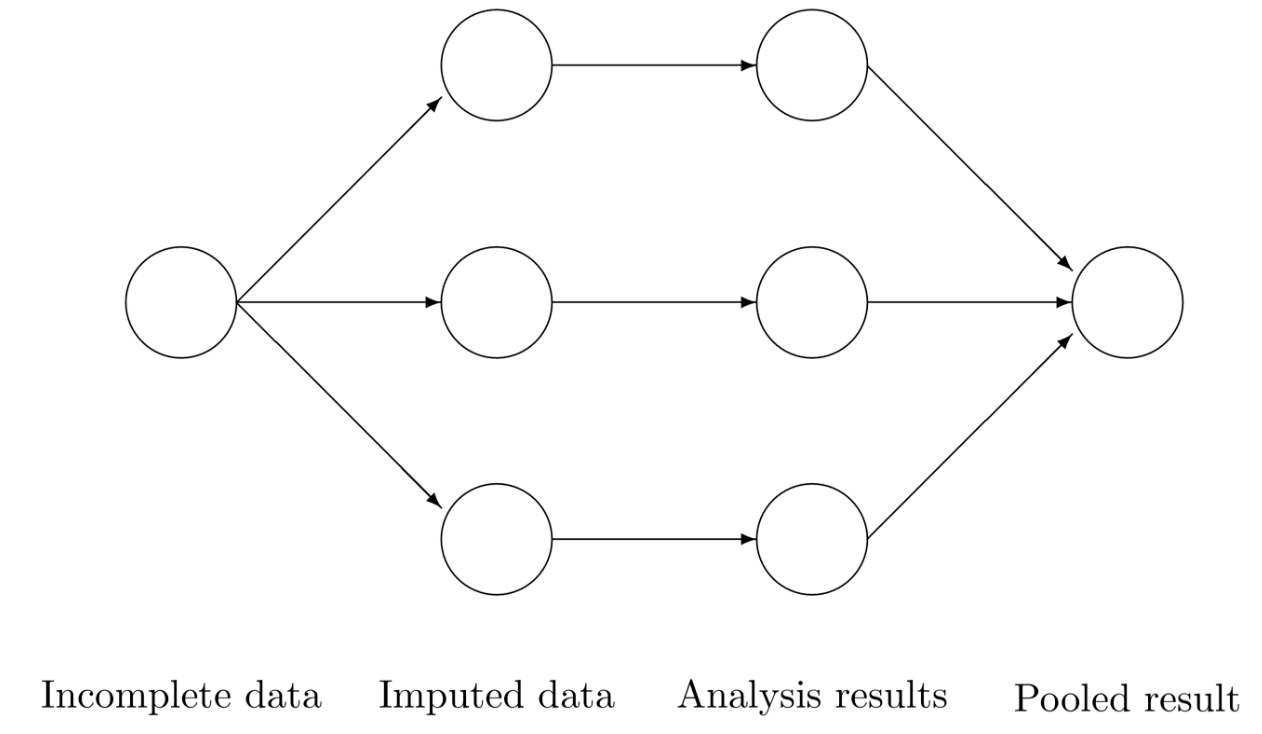
\includegraphics[width=400px]{figure/multiple-imputation-workflow} 

}

\caption{Multiple Imputation Workflow}\label{fig:mutlipleimputationworkflow}
\end{figure}
In multiple imputation, practitioners should choose an imputation method
that can produce sufficient variation for the imputed value between each
run. Then multiple imputation results in multiple copies of imputed
datasets with different imputed values. When performing analysis on
multiply imputed data, each imputed dataset is analyzed separately and
then parameters from those analyses are pooled together to get combined
diagnostics on the performance of the multiple imputation process and
the specified imputation model (Vink). This method ``solves the standard
error problem by calculating the variance of each parameter estimate
across the several data sets'' (Allison, 2012). The pooled parameters
replace those from the supervised machine learning model of interest.
The pooled parameters not only produce the coefficient estimate but also
the properly account for the increase in standard error due to
uncertainty introduced from imputing missing data.

The authors cover the analysis on multiply imputed data at the end of
this section. First, the authors focus on the differences between single
and multiple imputation in the context of imputation alone.

\section*{Single Imputation vs.~Multiple Imputation
Revisited}\label{background-example}
\addcontentsline{toc}{section}{Single Imputation vs.~Multiple Imputation
Revisited}

The example below helps visualize the inherent differences between the
single and multiple imputation procedure. Imagine a subset of the
complete data matrix \(Y\) from the weigh scale experiment:

\[Y_{subset}=\begin{bmatrix}soft & 60 \\ soft & NaN \\ soft & 65 \\ hard & 85 \\ hard & 90 \\ hard & NaN \end{bmatrix}\]

Further, assume the underlying missing data mechanism is ignorable, so
imputation focuses on the observed dataset only. From the matrix above,
one can discern that the distibution of weight depends on the surface of
the scale. In this example, \(P(Y_{weight}|Y_{surface}=soft)\)
\textasciitilde{} \(N(60, 5)\), and \(P(Y_{weight}|Y_{surface}=soft)\)
\textasciitilde{} \(N(90, 5)\). The figure below visualizes the
differences in the distribution of weight, conditional on the surface of
the scale.
\begin{figure}

{\centering 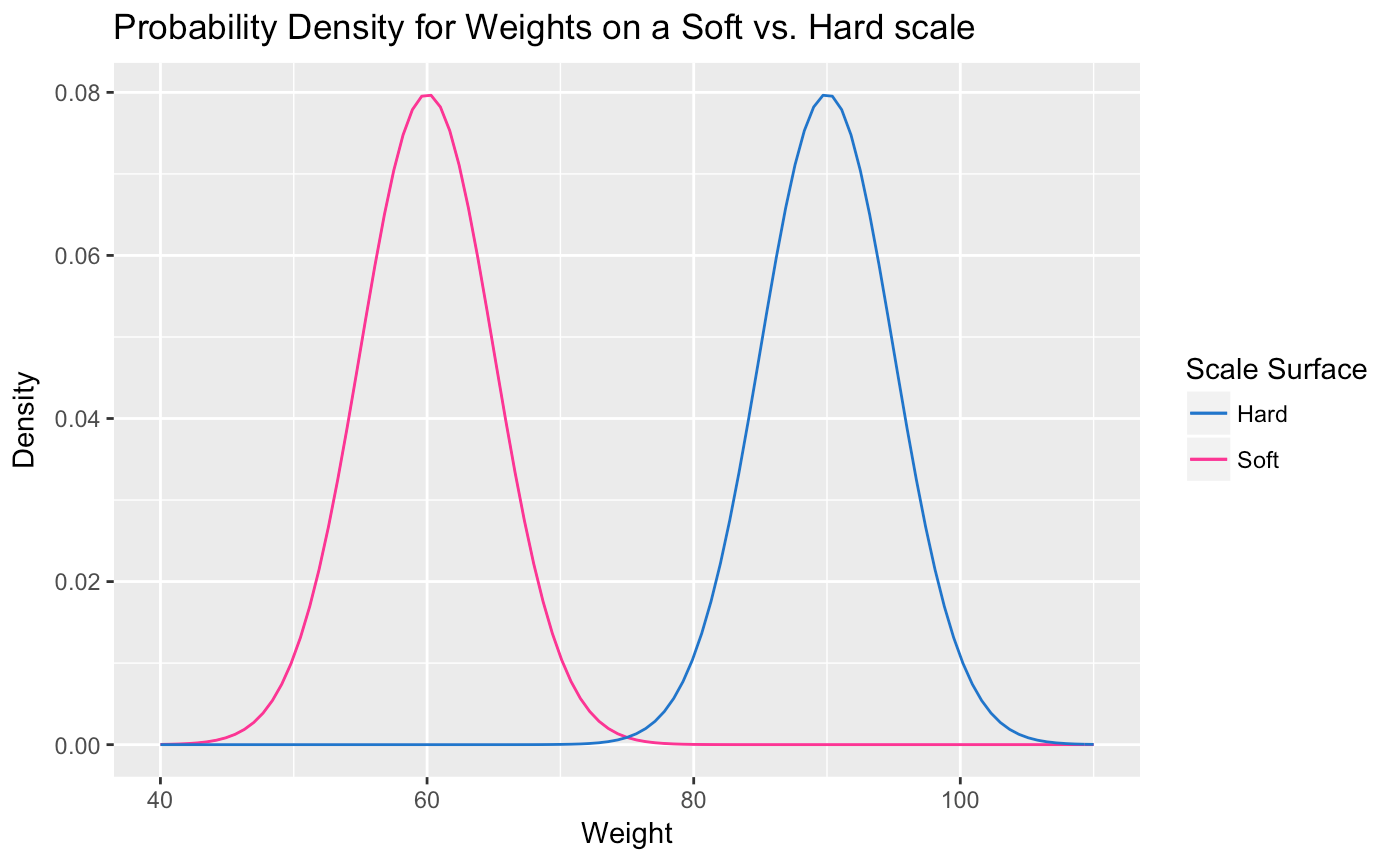
\includegraphics[width=400px]{figure/scale-distribution} 

}

\caption{Distribution of Weight by Scale Surface}\label{fig:scale-distribution}
\end{figure}
Now proceed with imputation analysis using single imputation. Assume
that the imputation models takes a random draw from each respective
surface's weight distribution to impute missing data. Then the complete
matrix becomes:

\[Y_{mis}=\begin{bmatrix}soft & 60 \\ soft & NaN \\ soft & 65 \\ hard & 85 \\ hard & 90 \\ hard & NaN \end{bmatrix} \rightarrow Y_{complete}=\begin{bmatrix}soft & 60 \\ soft & 63 \\ soft & 65 \\ hard & 85 \\ hard & 90 \\ hard & 91 \end{bmatrix}\]

The imputation model imputed 63 for \(Y_{2,2}\) and 91 for \(Y_{6,2}\).
Under single imputation, the matrix is now complete, as values for
weight have been imputed. But an analysis model has access to the
complete data matrix only, so it would not be able to distinguish which
values were imputed and which were originally observed. Therefore, an
analysis model treats the imputed values (63, 91) the same as observed
values. The imputed values carry no uncertainty with them into the
analysis phase.

Under multiple imputation, where \(m=3\) representing 3 imputations, the
matrices may look like the below:

\[Y_{mis}=\begin{bmatrix}soft & 60 \\ soft & NaN \\ soft & 65 \\ hard & 85 \\ hard & 90 \\ hard & NaN \end{bmatrix} \rightarrow Y_{complete}=\begin{bmatrix}soft & 60 \\ soft & 63 \\ soft & 65 \\ hard & 85 \\ hard & 90 \\ hard & 91 \end{bmatrix}, \begin{bmatrix}soft & 60 \\ soft & 66 \\ soft & 65 \\ hard & 85 \\ hard & 90 \\ hard & 89 \end{bmatrix},
\begin{bmatrix}soft & 60 \\ soft & 59 \\ soft & 65 \\ hard & 85 \\ hard & 90 \\ hard & 94 \end{bmatrix}\]

Multiple imputation produced 3 datasets. Across each imputation, the
observed have the same values, which makes sense given that the true
value of these weights is known. The imputed values, however, are
different. The differences reflect the uncertainty about the nature of
the true value imputed, given that the true value is actually missing.
Single imputation disregards this inherent variability, which tricks
analysis models into believing that the imputed values are true
observations. Multiple imputation retains the variability introduced by
the imputation process. This research covers analysis of multiply
imputed data in the next section, as there is some additional work
supervised learning methods must perform under multiple imputation. That
being said, it's important to take away the purpose of multiple
imputation. It not only retains the full sample size but also retains
the variability produced from the process of imputing missing data.

\section*{Analysis Models}\label{background-analysis}
\addcontentsline{toc}{section}{Analysis Models}

The primary purpose of handling missing data is to enable analysis
models to run. As previously noted, most supervised maching learning
models require datasets to be complete in order to fit an analysis model
capable of making predictions or classifications (Dong \& Peng, 2013).
The previous sections in the background address the main points a
researcher must consider when dealing with missing data. These
considerations influence the imputation model a researcher deploys to
impute missing data. The results from the imputation model then affect
the results produced from an analysis model run on imputed data.

One must remember that listwise deletion and imputation methods
fundamentally alter a dataset. Therefore, the quality of the results
produced from a missing data method depend on the degree to which the
method is able to capture the nature of the missing data when modeling
missing values (Vink). If the missing data method used is misspecified,
the structure of the data after imputation is distorted, and this
distortion affects inference derived from analysis models fit on the
altered dataset. This section addresses the impact of listwise deletion
and imputation from the perspective of analysis. It also covers the
additional work necessary to fit analysis models on multiply imputed
data.

In this research, an analysis model is nothing more than a supervised
machine learning method. This text focuses on linear and logistic
regression. Both techniques operate under the assumption that the
underlying dataset is complete, containing no missing records. As a
result, analysis models do not have any information regarding what
happened to the dataset before the model is fit. They cannot separate
imputed values from true observations, and they do not know if records
were removed through listwise deletion prior to analysis. Therefore, the
inference from the analysis model depends on the way in which missing
data is handled.

\subsection*{Analysis after Listwise
Deletion}\label{background-analysis-listwise}
\addcontentsline{toc}{subsection}{Analysis after Listwise Deletion}

In the \protect\hyperlink{background-deletion}{Deletion section}, the
authors explain the potential pitfalls associated with listwise
deletion. Depending on the proportion of missing data, listwise deletion
may significantly deplete the sample size on which an analysis model is
trained. In doing so, an analysis model generates larger standard errors
for parameters' estimates than it would had the dataset retained every
record in othe original sample. As a result, the significance of
coefficients may be called into question. Additionally, if the missing
data mechanism is not MCAR, listwise deletion may discard records which
contain important information. Doing so may lead to biased coefficient
estimates in addition to increased standard errors of those estimates
(Dong \& Peng, 2013).

While listwise deletion can cause problems downstream in analysis, there
are cases in which the method is appropriate for handling missing data.
Allison (2014) defends listwise deletion as a potentially optimal
solution under certain missing data patterns. Four cases in which
listwise deletion may outerperform more complex imputation methods
include the following:
\begin{itemize}
\tightlist
\item
  The proportion of missingness is very low relative to proportion of
  observed, and the sample size is large enough where loss of power is
  negligible.
\item
  The missing data mechanism is MCAR.
\item
  In linear regression, the missing data occurs in the \emph{predictor}
  variable only, regardless of the missing data mechanism, so long as
  the missingness does not depend on the \emph{response} variable used
  in an analysis model.
\item
  For logistic regression, the missing data occurs in the
  \emph{response} variable only, regardless of the missing data
  mechanism, so long as the missingness does not depend on the
  \emph{predictor} variables used in the analysis model.
\end{itemize}
Allison has proved that listwise deletion actually outerperforms other
methods, producing unbiased estimates so long as the regression models
are correctly specified and the criteria above are met (2014). That
being said, the practicioner should still benchmark listwise deletion
against other imputation methods, as the outcome from listwise deletion
is intricately linked to the nature of the missingness in the specific
dataset at hand.

\subsection*{Analysis after Single
Imputation}\label{background-analysis-single}
\addcontentsline{toc}{subsection}{Analysis after Single Imputation}

In the \protect\hyperlink{background-single-imputation}{Single
Imputation section}, the authors note that single imputation retains the
full dataset but ignores any uncertainty or variation introduced when
imputing missing values. Therefore, an analysis model such as linear
regression treats the single-imputed dataset as if each observation is a
true value. The analysis model fits the dataset as it would any other
dataset (van Buuren, 2018, ch.~2.1.2).

In the best case, if the imputation model used to impute data is not
misspecified, then the the coefficients produced from the analysis model
should at least be unbiased estimates of the true parameters had the
dataset been fully observed. In the worst case, the imputation model
used to impute data is misspecified, and the imputed values do not
accurately reflect the distribution of the missing data. In this case,
the analysis model produces coefficients that may be biased depending on
the severity of the imputation model's impact. In either situation, the
standard error of the estimates produced from the analysis model will be
too low (Gelman \& Hill, 2017, p.~532). When the standard error of a
parameter estimate is too low, the test-statistic for that parameter
will be too high, and the statistical significance of the parameter may
be inflated.

Underestimated standard errors may lead a researcher to erroneously
conclude that statistical relationships exist. Such inference is
dangerous and undermines the reason why missing data must be handled in
the first place. Even if the researcher understands the missing data
mechanism and applies a proper imputation model to handle missing data,
he or she may not have done enough to properly account for the
uncertainty introduced from imputation. That lack of consideration
appears downstream, affecting the ability for the researcher to trust
the significance of parameters from analysis models.

\subsection*{Analysis after Multiple
Imputation}\label{background-analysis-multiple}
\addcontentsline{toc}{subsection}{Analysis after Multiple Imputation}

To handle the problems incurred from single imputation, the authors
suggests researchers employ imputation methods using multiple
imputation. Multiple imputation creates multiple instances of the same
dataset, depending on the number of imputations specified. Each imputed
dataset has the same values for the observed but different imputations
for the missing values. These differences highlight the variability
introduced by imputation methods since the true value of a missing
observation is unknown (van Buuren, 2018, ch.~2.1.2).

While multiple imputation retains sample size and imputation
variability, it complicates the process of analysis. Because multiple
imputed datasets exist, the researcher cannot simply apply one model to
the complete dataset. Instead, the practicioner must apply the same
supervised model independently to each imputed dataset and then pool the
results of each analysis model to produce proper coefficient estimates
and standard errors.

The authors introduce new notation to explain the pooling process used
in multiple imputation. Again, the authors follow the notation outlined
in van Buuren. The notation in this section also appears in Appendix B,
the expressions appear in Appendix C, and concepts appear in Appendix D.

Assume \(Q\) is the population parameter of interest. In the context of
analysis models, \(Q\) is a scalar for the \(\beta\) coefficient from
simple linear regression or a vector \(\vec{Q}\) containing the
\(\beta_1,...,\beta_p\) coefficients from multiple linear regression.
(Note the same notation applies to coefficients from other regression
models, such as logistic regression). In either case, \(\hat{Q}\) is the
estimate of \(Q\). \(U\) represents the variance of estimate \(\hat Q\)
or the covariance matrix of \(\vec{\hat Q}\) (van Buuren, 2018,
ch.~2.3.).

In the case of complete data or single imputation, the researcher fits
an analysis model and produces the estimate \(\hat{Q}\). But when the
researcher uses multiple imputation, the researcher must apply the
analysis model to each imputed datset independently. Therefore, the
researcher ends up with \(m\) x \(\hat{Q}\) estimates and \(m\) x \(U\)
covariance matrices, one set from each analysis model applied to \(m\)
imputed datasets (van Buuren, 2018, ch.~2.3). The researcher must pool
these parameters together to build one analysis model that properly
accounts for the estimates from each \(m\) imputed dataset.

Pooling the coefficient estimate is the most straightforward. The
equation is as follows:

\[\bar Q = \frac{1}{m}\sum_{\ell=1}^m \hat Q_\ell\] In this equation,
\(\bar Q\) is the average of the \(\hat Q\) estimates from each of the
\(m\) imputed datasets. This equation reduces the coefficients from each
imputed dataset down to one estimate (or vector of coefficients) by
taking the average across the \(m\) imputed datasets. The resulting
value is the pooled parameter estimate for the analysis model on
multiply imputed data.

Pooling variance is more involved. The researcher must account for the
variance from the analysis model of each imputed dataset. Additionally,
the researcher must account for the variance that occurs between \(U\)
from each analysis model. Lastly, the researcher must add extra variance
to account for the fact that only \(m\) imputations were performed.

The first formula is the variance within:

\[ \bar U = \frac{1}{m}\sum_{\ell=1}^m \bar U_\ell\] This formula is
called \textbf{variance within}. As with the coefficient estimate,
variance within is the average of the variance within each of the
analysis models fit on the \(m\) imputed datasets. It is the traditional
variance metric one would expect from a linear regression, expect in the
case of multiple imputation, it is the average across the \(m\) imputed
datasets (van Buuren, 2018, ch 2.3).

The next formula is the variance between:

\[B = \frac{1}{m-1}\sum_{\ell=1}^m (\hat Q_\ell-\bar Q)(\hat Q_\ell-\bar Q)'\]
This equation is called \textbf{variance between}. Because each of the
\(m\) imputed datasets produces a separate set of estimates for
\(\hat Q\), variance exists between the estimates of each imputed
dataset. Therefore, the analysis must account for the variance that
occurs between the different estimates each imputation procedure
produces (van Buuren, 2018, ch 2.3).

The final formula represents the total variance:

\[T = \bar U + B + B/m\] This equation is the \textbf{total variance}
for the pooled parameter estimate of \(\bar Q\). It adds the variance
within to the variance beween to the additional variance from a finite
number of imputations, \(m\). Note that as \(m \rightarrow \infty\), the
last part of this equation goes to \(0\). But because one cannot perform
an infinite number of imputations, additional variance must be added to
account for the number of imputations the researcher conducts (van
Buuren, 2018, ch.~2.3).

Therefore, the analysis model for multiply imputed data is parameterized
by \(\bar Q\) and \(T\). These parameters pool each individual analysis
model applied to \(m\) imputed datasets and produce one analysis model
that accurately measures the coefficient estimate and accounts for the
variance that results from imputing data.

While the process is more involved, analysis of multiply imputed data
fully captures the impact of missingness and the effect of imputation.
The pooled parameters also provide insights into the efficiency and
performance of the imputation process. For example, a large variance
between metric indicates that the imputation model produces wildly
different imputations for each dataset. As a result, the analysis model
produces largely different coefficient estimates, so the variance
between them is high.

\section*{Missing Data and
Autoimpute}\label{background-missing-data-autoimpute}
\addcontentsline{toc}{section}{Missing Data and Autoimpute}

This background explores the main concepts related to missing data and
discusses what a researcher must consider before selecting which missing
data method to use. The section then introduces numerous missing data
methods, each of which operates with its own set of assumptions but all
of which assume that the missing data mechanism is at least ignorable.
This text then briefly examines the impact of deletion and imputation on
supervised analysis and demonstrates how concepts from missing data can
leak into the inference of an analysis model if missingness is not
handled with care.

The \texttt{Autoimpute} package gives the end user the tools to step
through the entire process of handling missing data to performing
supervised analysis. The package includes methods to explore and
visualize missing data to discern what missing data mechanisms may be
present. The package also includes numerous imputation methods, which
the practicioner can use within the package's implementation of the
Single Imputation and Multiple Imputation frameworks. Finally,
\texttt{Autoimpute} extends linear and logistic regression to mulitply
imputed datasets. In doing so, \texttt{Autoimpute} handles parameter
pooling and variance calculation for the user. It also includes
additional metrics and diagnostics to assess the impact of imputation on
downstream analysis.

In the Methodology section, the authors return to the
\texttt{Autoimpute} package itself and demonstrate how it is used to
step through everything covered in the background section. In addition,
the authors design experiments to dig deeper into the effect of specific
imputation models and how they affect analysis depending on the nature
of the missing data.

\hypertarget{methodology}{\chapter*{Methodology}\label{methodology}}
\addcontentsline{toc}{chapter}{Methodology}

The missing data methods introduced in the background section are a
subset of those available in \texttt{Autoimpute}. Beyond
\texttt{Autoimpute} numerous additional missing data methods exist to
handle missing data, and they are continuously being developed and
improved (Schouten, et al, 2018). Therefore, it is vital to understand
the circumstances under which each missing data method is effective, and
it is important to evaluate each technique in relation to other methods
(Schouten, et al, 2018). To do so, researchers can simulate complete
datasets then introduce artificial missingness under different types of
missing data mechanisms with different missing data patterns. Such a
procedure affords the researcher an opportunity to evaluate missing data
methods and their effect on analysis models under different
circumstances (Schouten, et al, 2018).

\hypertarget{methodology}{\section*{Assessing Missing Data Methods
through Simulation}\label{methodology}}
\addcontentsline{toc}{section}{Assessing Missing Data Methods through
Simulation}

Schouten, et al. (2018) formalizes a step-by-step process in which a
missing data methodology is evaluated by means of simulations:
\begin{enumerate}
\def\labelenumi{\arabic{enumi}.}
\tightlist
\item
  Simulate a multivariate, complete dataset. The complete dataset
  becomes the population of interest and the source of truth.
\item
  Introduce arificial missingness to the complete dataset using missing
  data mechanisms and missing data patterns. This process results in an
  incomplete dataset.
\item
  Use missing data methods to handle the missing data in the incomplete
  dataset.
\item
  Apply an analysis model and obtain statistical inference for the
  original, complete dataset as well as the incomplete dataset after
  dealing with the missing values. A comparison of these inferences
  gives an indication of the performance of the missing data method.
\end{enumerate}
In this methodology, the authors follow the steps outlined above. The
authors simulate a complete dataset using the \texttt{MASS} package in R
(Venables \& Ripley, 2002). The authors introduce missingness in a
complete dataset using the \texttt{ampute} function from the
\texttt{MICE} package in R (van Buuren \& Groothuis-Oudshoorn, 2011).
The \texttt{ampute} function can generate multivariate missing data
within a complete dataset by defining a missing data mechanism (MCAR,
MAR, MNAR) as well as missing data patterns, such as proportions of
missingness and the features that should contain missingness (van Buuren
\& Groothuis-Oudshoorn, 2011). The authors use these R packages to
produce complete and incomplete datasets, which cover steps 1 and 2
above.

Next, the authors use \texttt{Autoimpute} to cover steps 3 and 4. The
authors explore the performance of imputation methods and their effect
on analysis models under two separate circumstances. The authors begin
by simulating a dataset with no missingness. A simple linear regression
is performed on this simulated dataset and its parameters of interest
are stored as benchmarks. Next, the researchers create artifical
missingness in the complete dataset using two different types of missing
data mechanisms with different missing data patterns. This procedure
results in two disctinct, incomplete datasets. Each incomplete dataset
will have different observations missing, but any observed values will
be the same across the two incomplete datasets and the original complete
dataset.

The authors then impose the same deletion and impution methods on each
of the incomplete datasets. In each example, the researchers first
explore missingness patterns within the dataset. Then, the authors use
the following missing data methods:
\begin{itemize}
\tightlist
\item
  Listwise deletion or CCA
\item
  Mean imputation
\item
  Least Squares imputation
\item
  Predictive Mean Matching
\end{itemize}
Mean, least squares, and predictive mean matching are performed using
the mutliple imputation framework. Listwise deletion is performed
separately because it does not require single or multiple imputation.
All methods are implemented using the \texttt{Autoimpute} package.

\texttt{Autoimpute} offers many more missing data methods, but these
four are useful for this study because each carries a different set of
assumptions and takes a very different approach to handling missing
values. Listwise deletion is a deletion method, so it ignores
missingness entirely by discarding records with any missing
observations. Mean imputation is a univariate method, so it disregards
any structure between the target variable and other features. Least
squares is a supervised multivariate method that considers the structure
of the data but ignores the uncertainty surrounding imputation. Finally,
PMM is an advanced semi-supervised multivariate method that blends
concepts from bayesian analysis, linear regression, and k-nearest
neighbors. The sections below demonstrate when these methods work and
when they do not. As always, their performance is directly linked to the
missing data mechanism at hand and the nature of missingness within a
dataset. Therefore, some methods shine in circumstances where other
methods underperform.

\section*{The Full Dataset}\label{the-full-dataset}
\addcontentsline{toc}{section}{The Full Dataset}

The authors use the MASS package (Venables \& Ripley, 2002) to simulate
the full dataset, or the source of truth. The full dataset contains 500
observations for feature \(x\) and response \(y\). The dataset is
generated from a joint normal distribution, where \(\mu_x=10\) and
\(\mu_y=5\). The correlation between \(x\) and \(y\) equals 0.7. At this
point, no missingness exists in \(x\) or \(y\).

The figure below visualizes the distribution of each variable:
\begin{figure}

{\centering 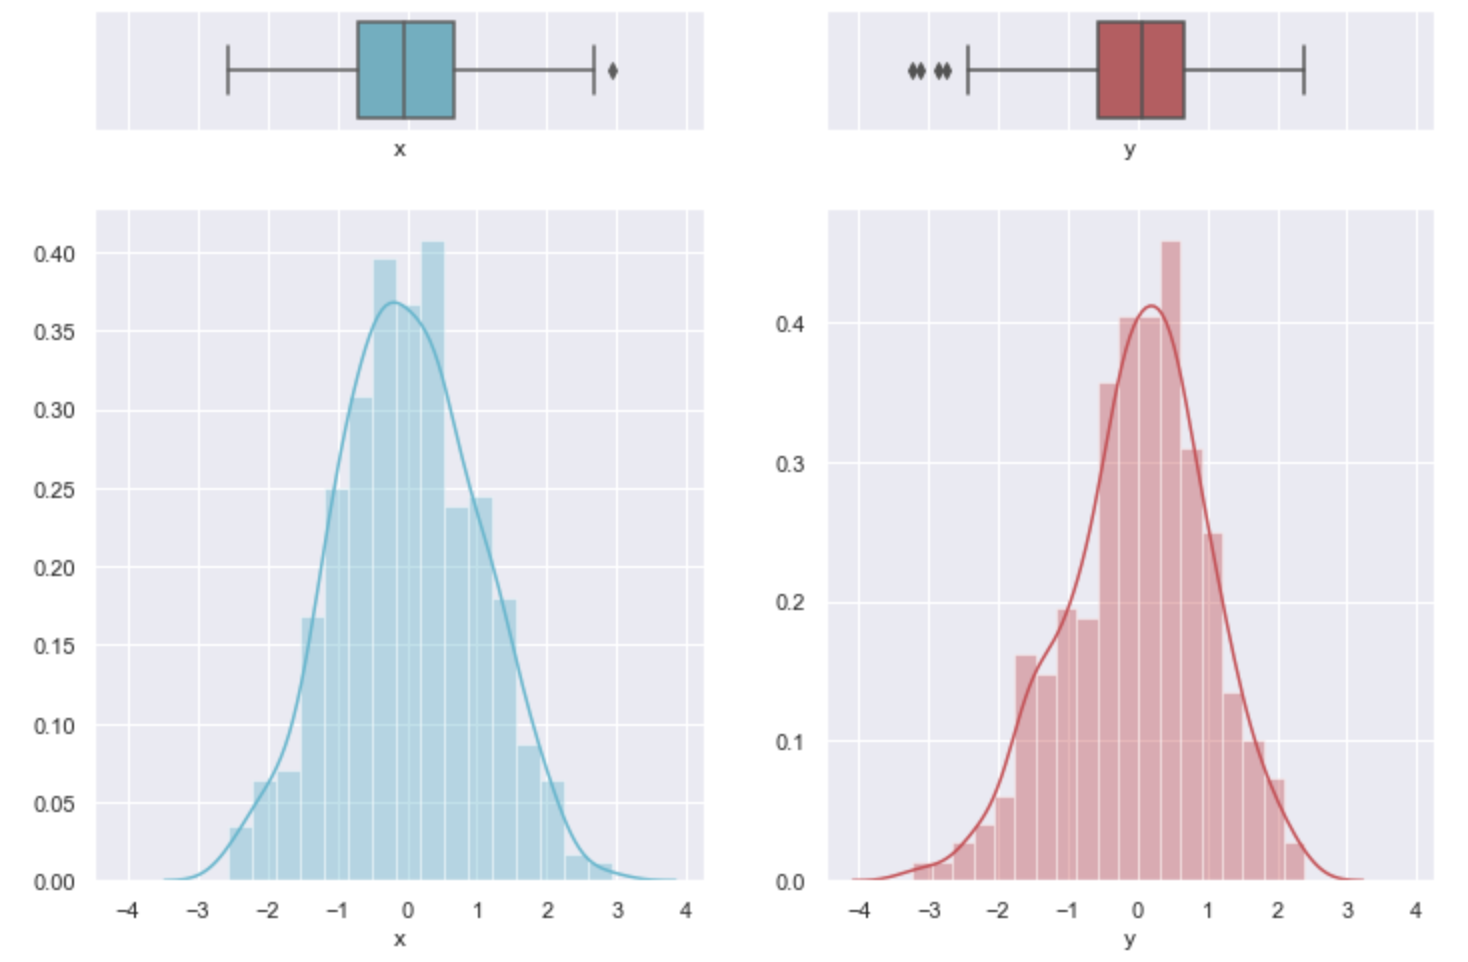
\includegraphics[width=400px]{figure/full-side-by-side} 

}

\caption{Distribution of Full x and y}\label{fig:fullsidebyside}
\end{figure}
The next figure displays the joint relationship between \(x\) and \(y\).
The figure plots the marginal distribution of each variable as well:
\begin{figure}

{\centering 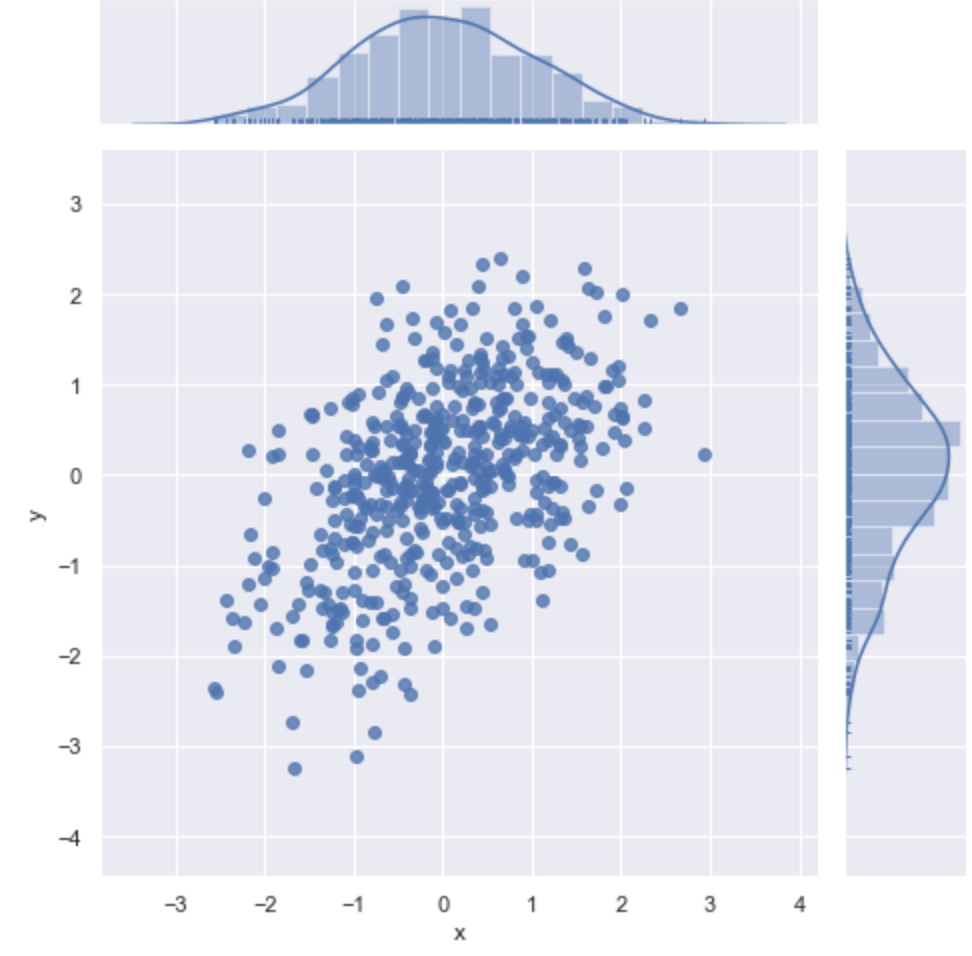
\includegraphics[width=400px]{figure/full-joint} 

}

\caption{Joint and Marginals of Full x and y}\label{fig:full-joint}
\end{figure}
Both plots come from native visualization methods in the
\texttt{Autoimpute} package.

The full dataset does not contain any missing values, so no deletion or
imputation is necessary before conducting analysis. Using
\texttt{Autoimpute}, the researchers fit a linear regression model on
the full dataset. The summary of the model fit appears below:
\begin{figure}

{\centering 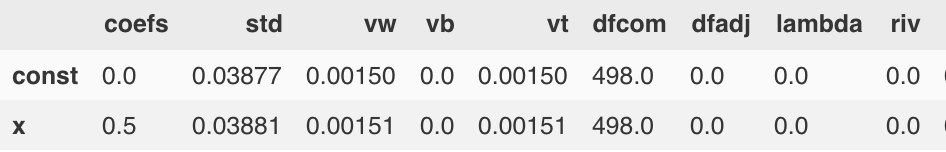
\includegraphics[width=400px]{figure/full-regression} 

}

\caption{Linear Regression Results: Full}\label{fig:full-regression}
\end{figure}
The results from linear regression on the full dataset serve as the
golden source. The coefficient estimate for \(x\) is 0.7. Using notation
related to imputation analysis, this coefficient estimate of \(x\)
represents \(\hat Q\) - the unbiased estimate of the population
parameter of interest \(Q\). Because there is only one predictor, the
covariance matrix \(U\) simply reduces to the variance of the estimate.

The summary output above displays diagnostics for the linear regression
model. The output uses aliases for concepts covered in the
\protect\hyperlink{background}{Background section}
\begin{itemize}
\tightlist
\item
  \texttt{coefs} - The parameter estimate \(\hat Q\)
\item
  \texttt{std} - The standard error of the coefficient estimate
\item
  \texttt{vw} - The variance-within \(\bar U\)
\item
  \texttt{vb} - The variance-between \(B\)
\item
  \texttt{vt} - The total variance \(T\)
\end{itemize}
Observe that \texttt{vb}, or the variance-between, is equal to 0. This
result occurs because no missingness exists and multiple imputation is
not used. The variance-between becomes important in subsequent sections
where missing data methods are used within the multiple imputation
framework.

\section*{Example 1: MCAR with Missingness in the
Response}\label{example-1-mcar-with-missingness-in-the-response}
\addcontentsline{toc}{section}{Example 1: MCAR with Missingness in the
Response}

In the first example, the researchers generate MCAR missingness within
the response, \(y\). Response \(y\) contains 40\% missing values.
Feature \(x\) remains fully observed. The two plots below showcase how
to use \texttt{Autoimpute} to explore missingness within a given
dataset. \texttt{Autoimpute} leverages the excellent \texttt{missingno}
python package to explore missingness within datasets (Bilogur, 2018)
prior to applying any missing data methods. The plots are quite simple
in this case, but they can help detect patterns in missing data when
multiple features are present with different levels of missingness.
\begin{figure}

{\centering 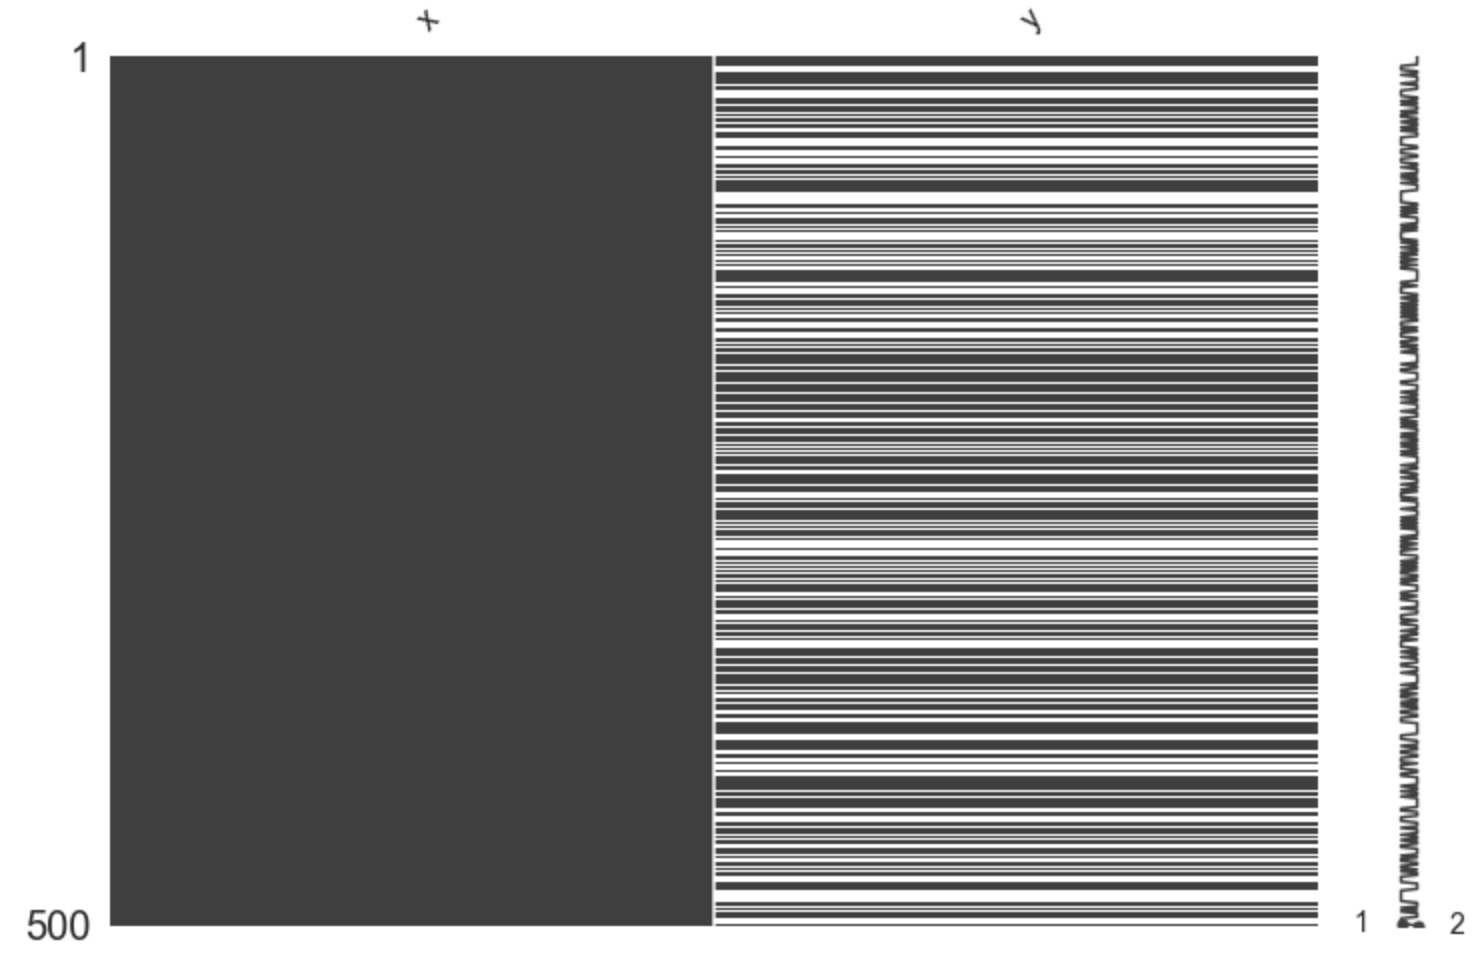
\includegraphics[width=400px]{figure/y-mis-forty-loc} 

}

\caption{Missingness Locations}\label{fig:y-mis-forty-loc}
\end{figure}
\begin{figure}

{\centering 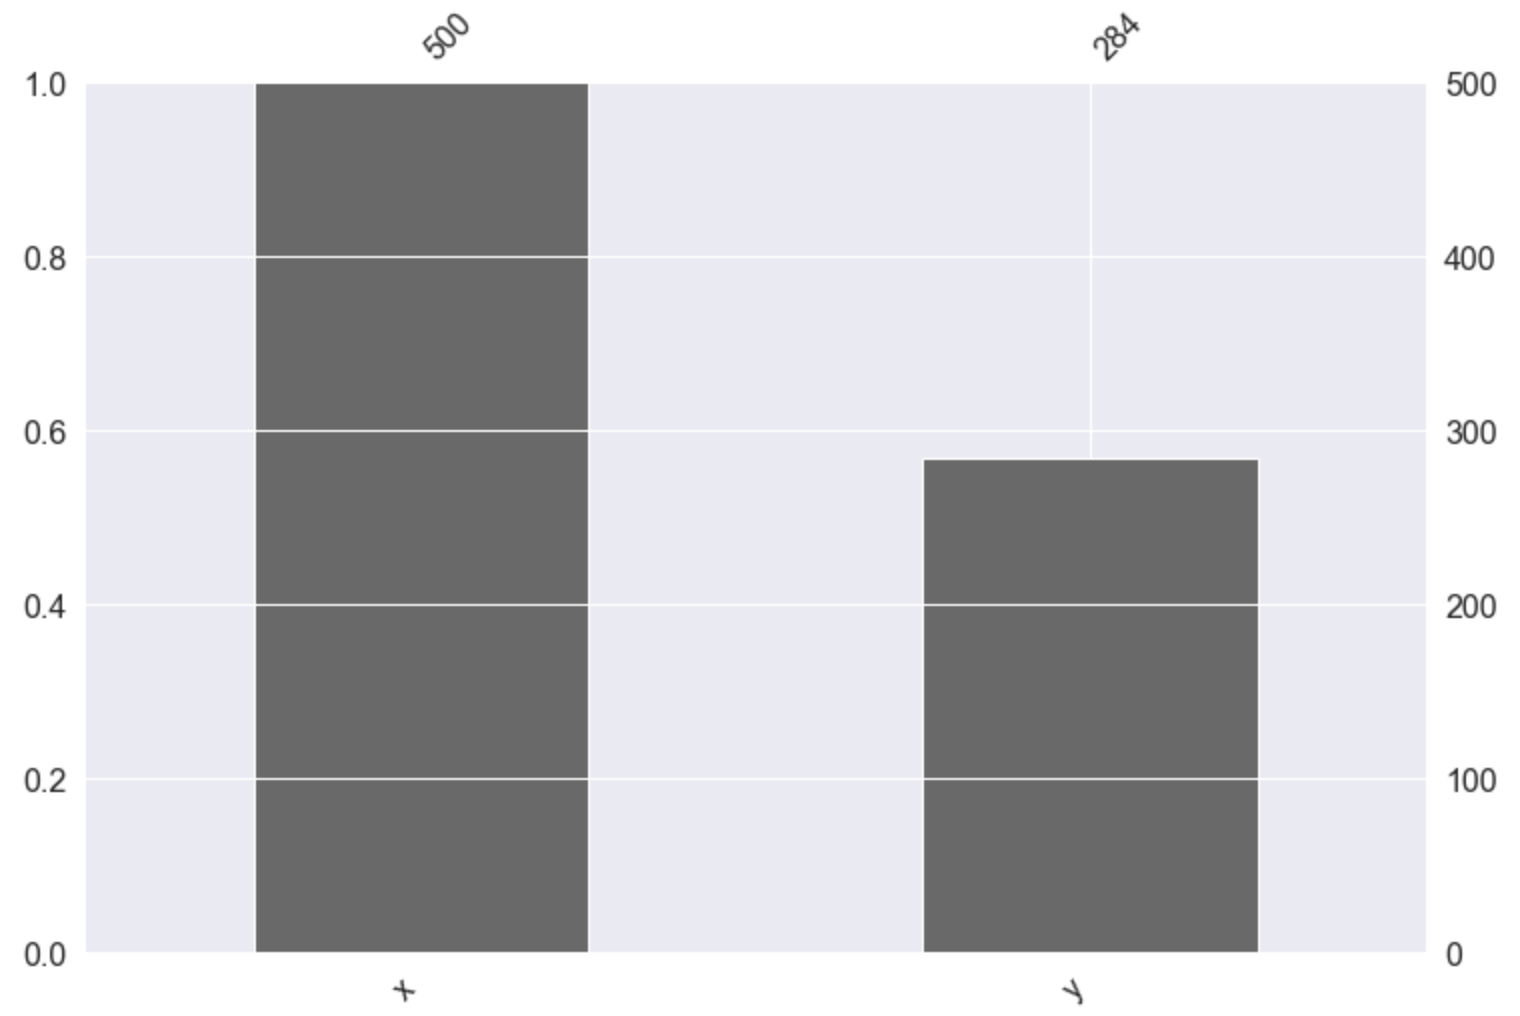
\includegraphics[width=400px]{figure/y-mis-forty-bar} 

}

\caption{Missingness Percentage}\label{fig:y-mis-forty-bar}
\end{figure}
Next, the researchers employ missing data methods to handle missing data
in \(y\). In this case, missing data methods must find plausible
imputations for the 40\% of \(y\) that is missing. The imputation
methods used include mean, linear regression, and pmm. The researchers
also use listwise deletion, although there is no visualization within
\texttt{Autoimpute} for complete-case analysis because no imputations
are performed. For imputation methods, the researchers deploy each
strategy within the multiple imputation framework. The number of
imputations performed for each method is 5.

\texttt{Autoimpute} supports a number of visualization metrics to assess
the impact of imputation on an incomplete dataset.

The visualizations below show the impact of mean, linear regression, and
pmm imputation. For each strategy, there are two respective plots. The
first plot is the new multivariate distribution between \(x\) and \(y\)
after imputation. The second plot shows the imputations for \(y\)
against other, observed values for \(y\) for each of the \(5\)
imputations performed.

Let's start with mean imputation:
\begin{figure}

{\centering 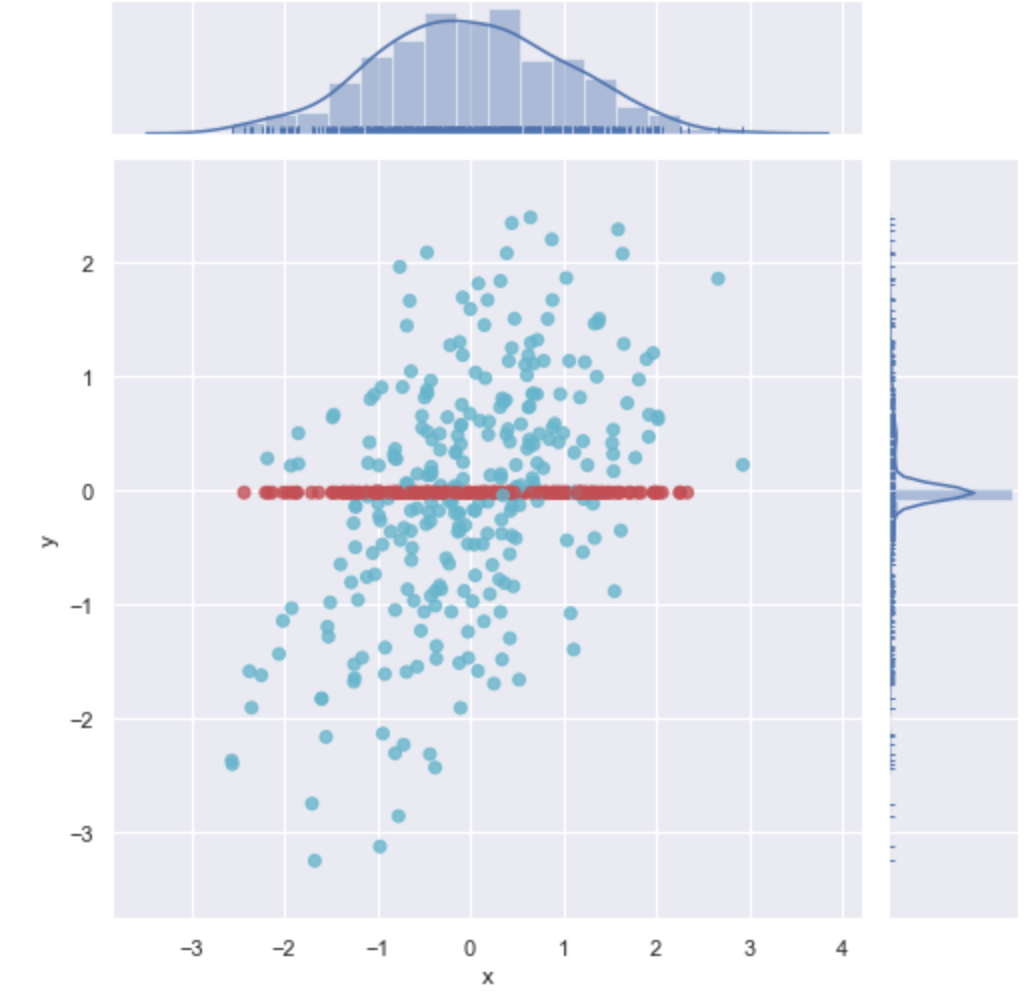
\includegraphics[width=400px]{figure/multi-mean} 

}

\caption{Joint and Marginals with Mean Imputation}\label{fig:multi-mean}
\end{figure}
\begin{figure}

{\centering 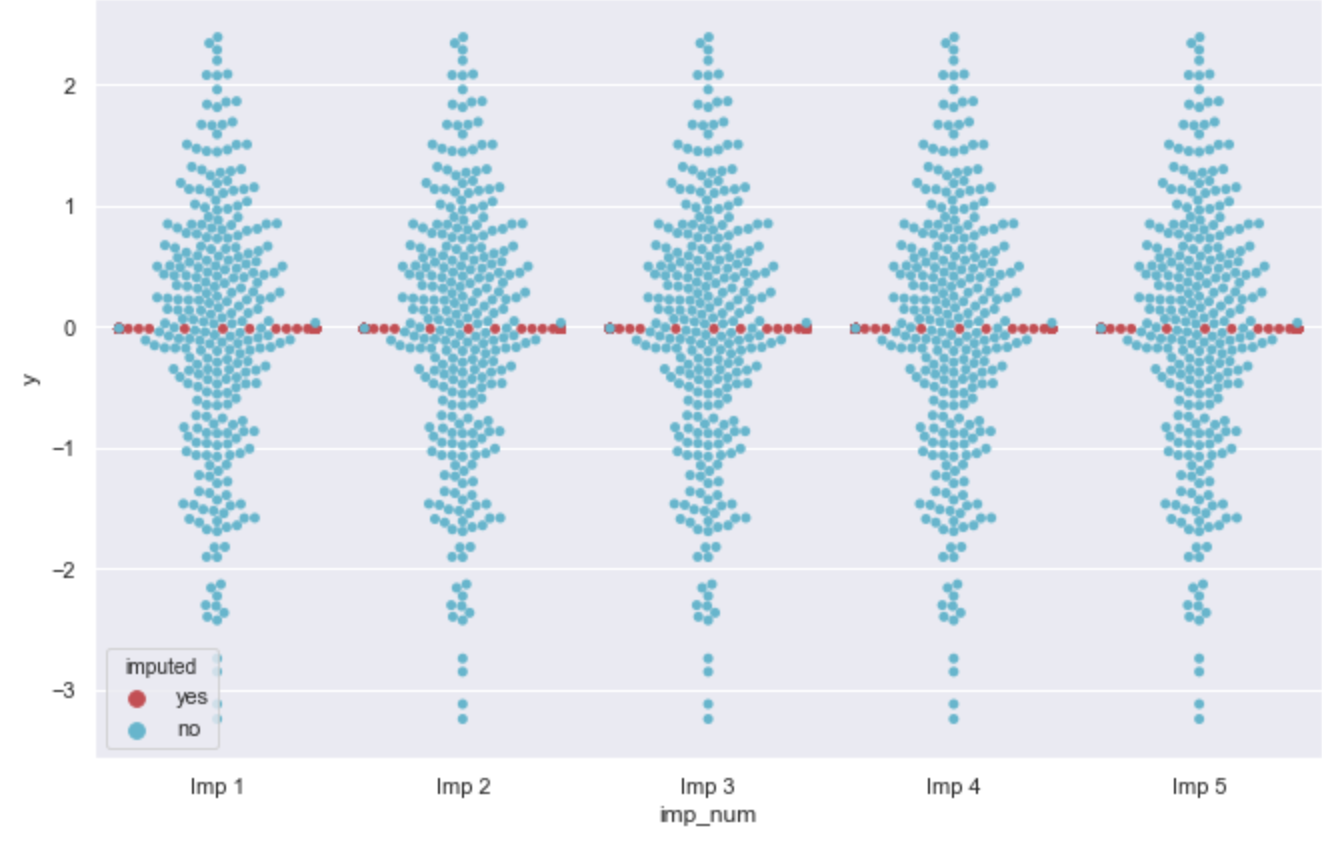
\includegraphics[width=400px]{figure/swarm-mean} 

}

\caption{Swarm Plot: Mean Imputation}\label{fig:swarm-mean}
\end{figure}
Note that for mean imputation, the imputations do not depend on the
value of \(x\), and the relationship between \(y\) and \(x\) is ignored.
This result makes sense, as mean imputation is a univariate method. Also
note that the imputation values in the swarm plot are the same for each
imputation. This occurs because the mean of the observed values of \(y\)
do not change from imputation to imputation within the multiple
imputation framework. Therefore, the imputation values within each
imputed dataset are the same, and the imputation values accross each
imputed dataset are the same.

Next, observe imputation via least squares:
\begin{figure}

{\centering 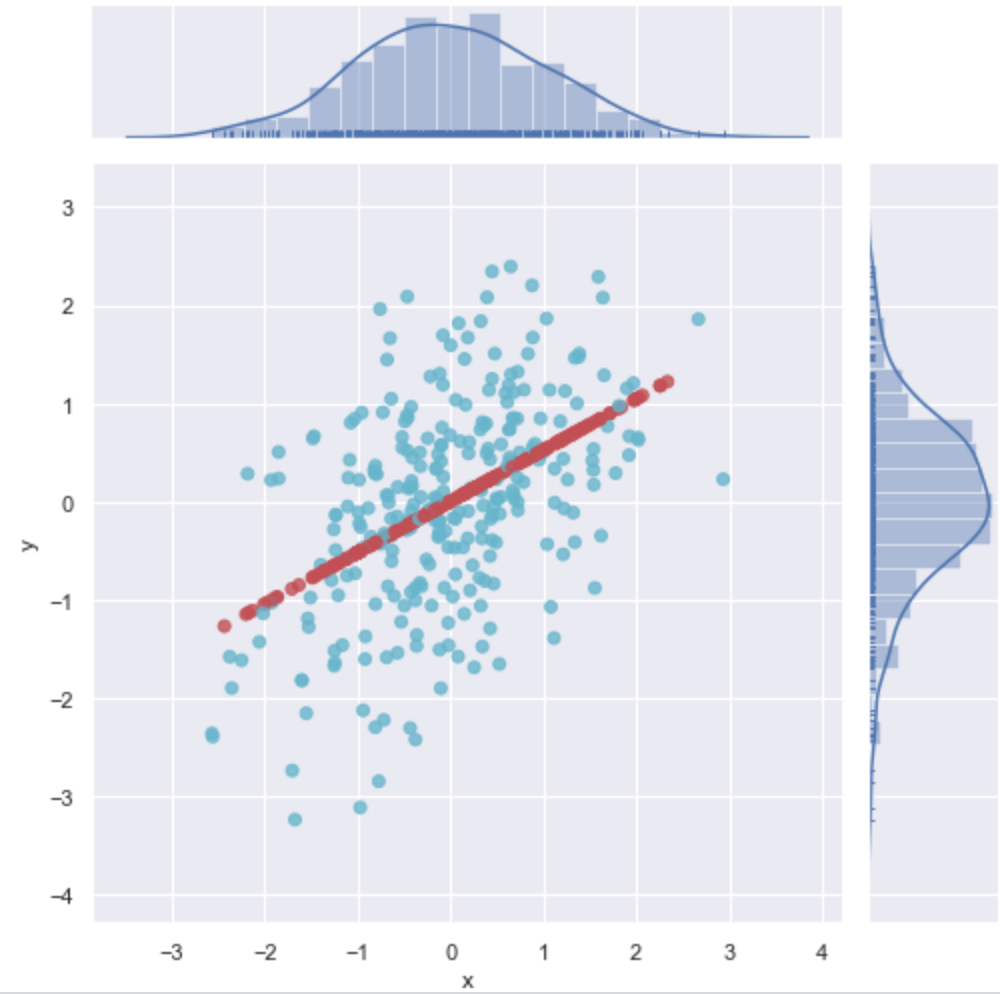
\includegraphics[width=400px]{figure/multi-lm} 

}

\caption{Joint and Marginals with Least Squares Imputation}\label{fig:multi-lm}
\end{figure}
\begin{figure}

{\centering 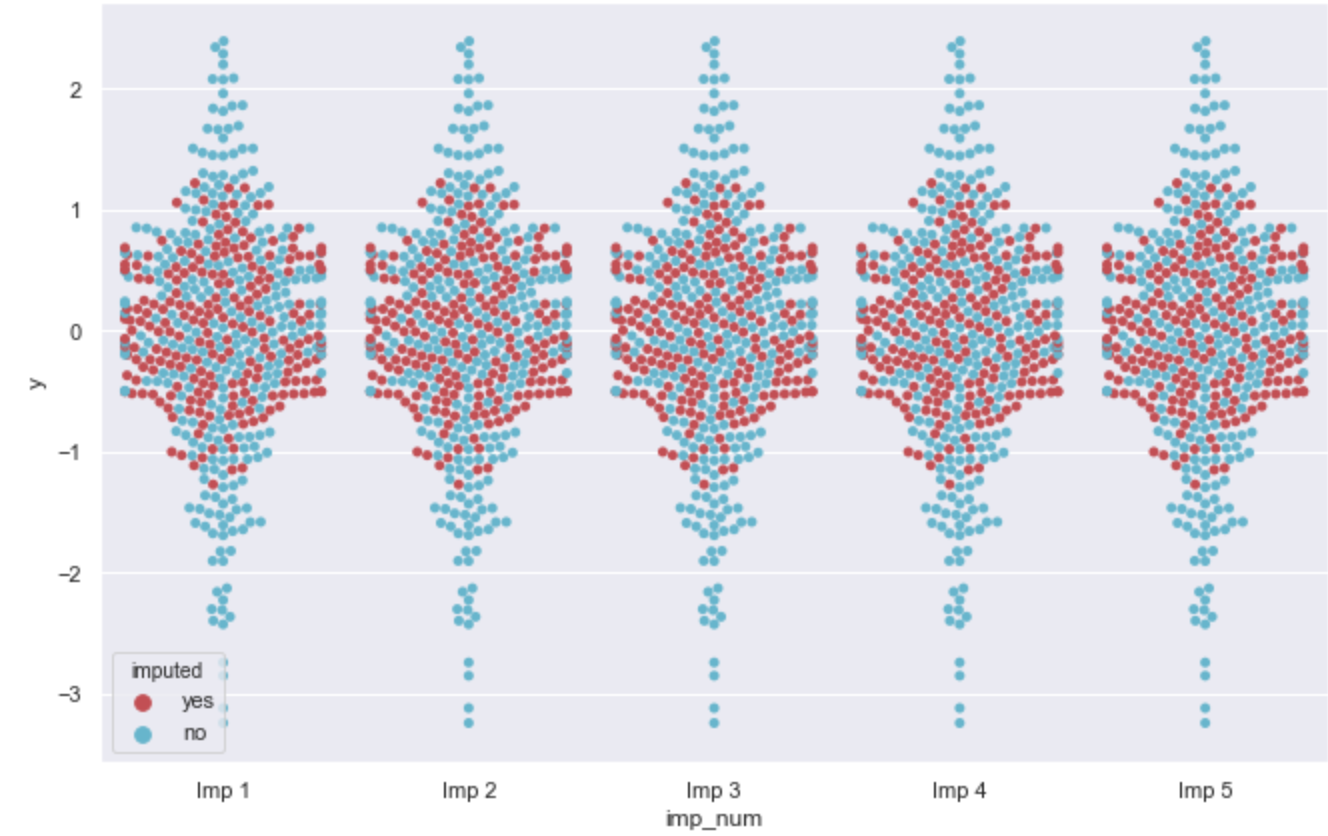
\includegraphics[width=400px]{figure/swarm-lm} 

}

\caption{Swarm Plot: Least Squares Imputation}\label{fig:swarm-lm}
\end{figure}
The plots for linear regression now take into account the relationship
between \(y\) and \(x\). As a result, the imputed values are different
within imputations but the same across imputations. Within an incomplete
dataset, the linear model produces different imputed values, which
depend on the value of \(x\). But across incomplete datasets, the linear
model's imputed values are the same because the model is fit on the same
observed data and no random error is added to imputations.

Finally, observe pmm imputation:
\begin{figure}

{\centering 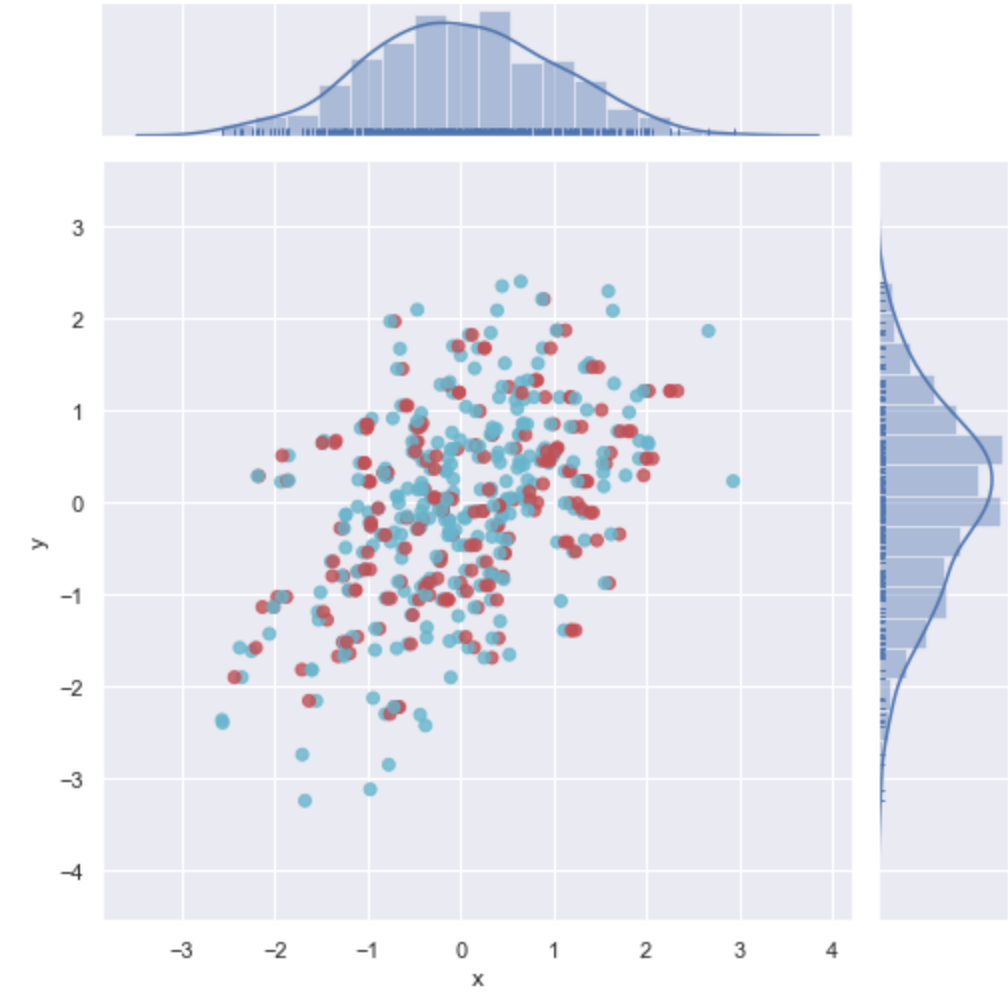
\includegraphics[width=400px]{figure/multi-pmm} 

}

\caption{Joint and Marginals with PMM Imputation}\label{fig:multi-pmm}
\end{figure}
\begin{figure}

{\centering 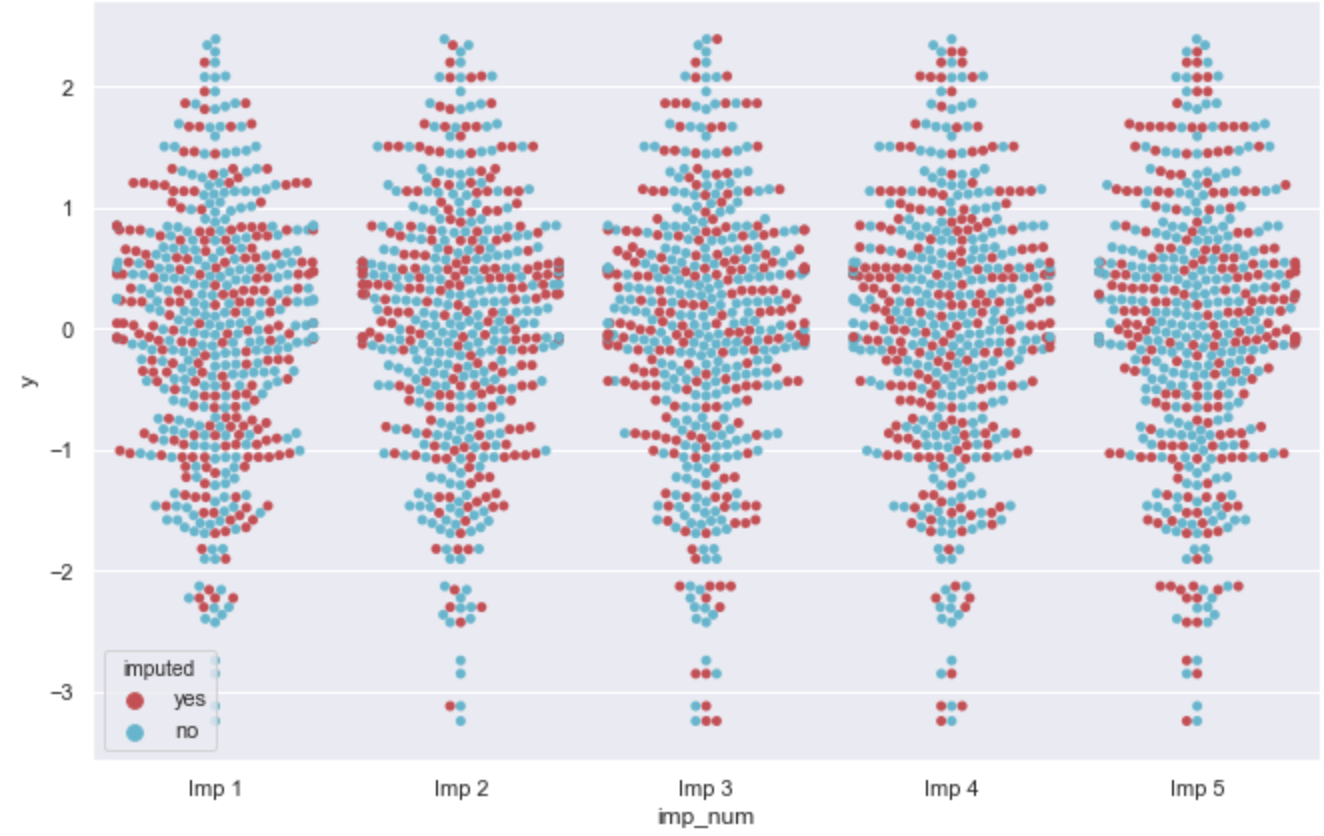
\includegraphics[width=400px]{figure/swarm-pmm} 

}

\caption{Swarm Plot: PMM Imputation}\label{fig:swarm-pmm}
\end{figure}
PMM Imputation respects not only the relationship between \(y\) and
\(x\) but also the variance between the features. Imputations are no
longer from the ``line of best fit'' as they are with linear regression.
Additionally, imputations are different within and across incomplete
datasets. Therefore, PMM does the best job at respecting the structure
of the data and adding variance between / across imputed datasets.

\section*{Example 2: MAR with Missingness in the
Predictor}\label{example-2-mar-with-missingness-in-the-predictor}
\addcontentsline{toc}{section}{Example 2: MAR with Missingness in the
Predictor}

In the second example, the researchers generate MAR missingness within
the predictor, \(x\). The missigness is right-tailed, which means that
the probability that predictor \(x\) is missing increases with the value
of \(y\). Predictor \(x\) contains 40\% missing values. Response \(y\)
remains fully observed.

The researchers take the same approach to Example 2 as they do to
Example 1. First, the authors plot the missing data patterns within
\(x\) and \(y\). Then, listwise deletion is performed, followed by
multiple imputation for mean, least squares, and predictive mean
matching. Again, the multiple imputation iterates 5 times.

The plots below demonstrate that missingness now occurs within the
predictor \(x\), while \(y\) is fully observed.
\begin{figure}

{\centering 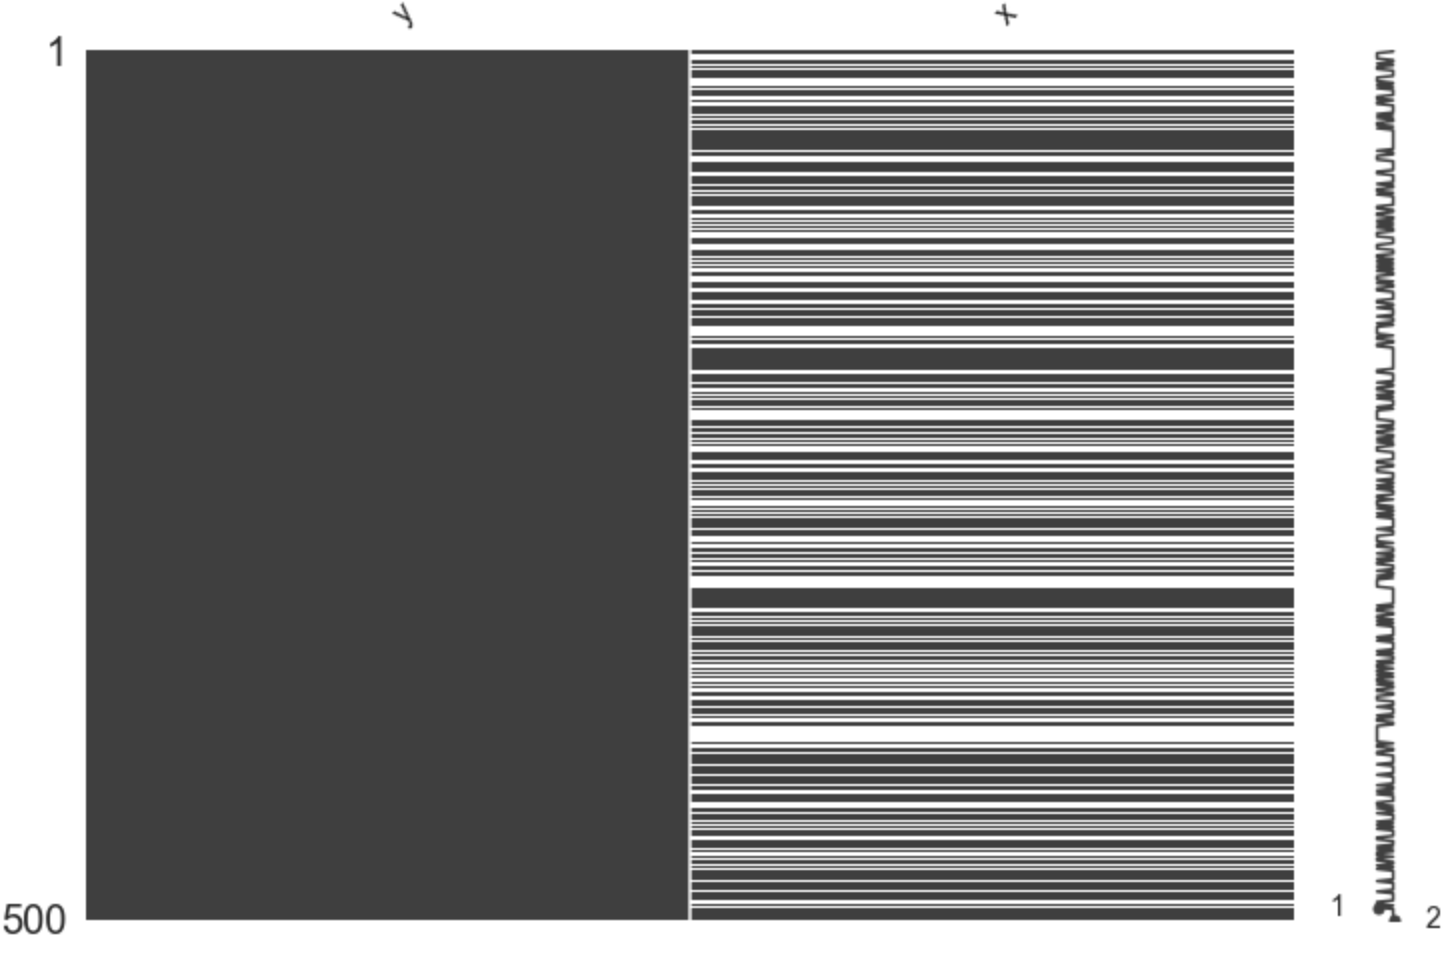
\includegraphics[width=400px]{figure/x-mis-forty-loc-mar} 

}

\caption{Missingness Locations}\label{fig:x-mis-forty-loc-mar}
\end{figure}
\begin{figure}

{\centering 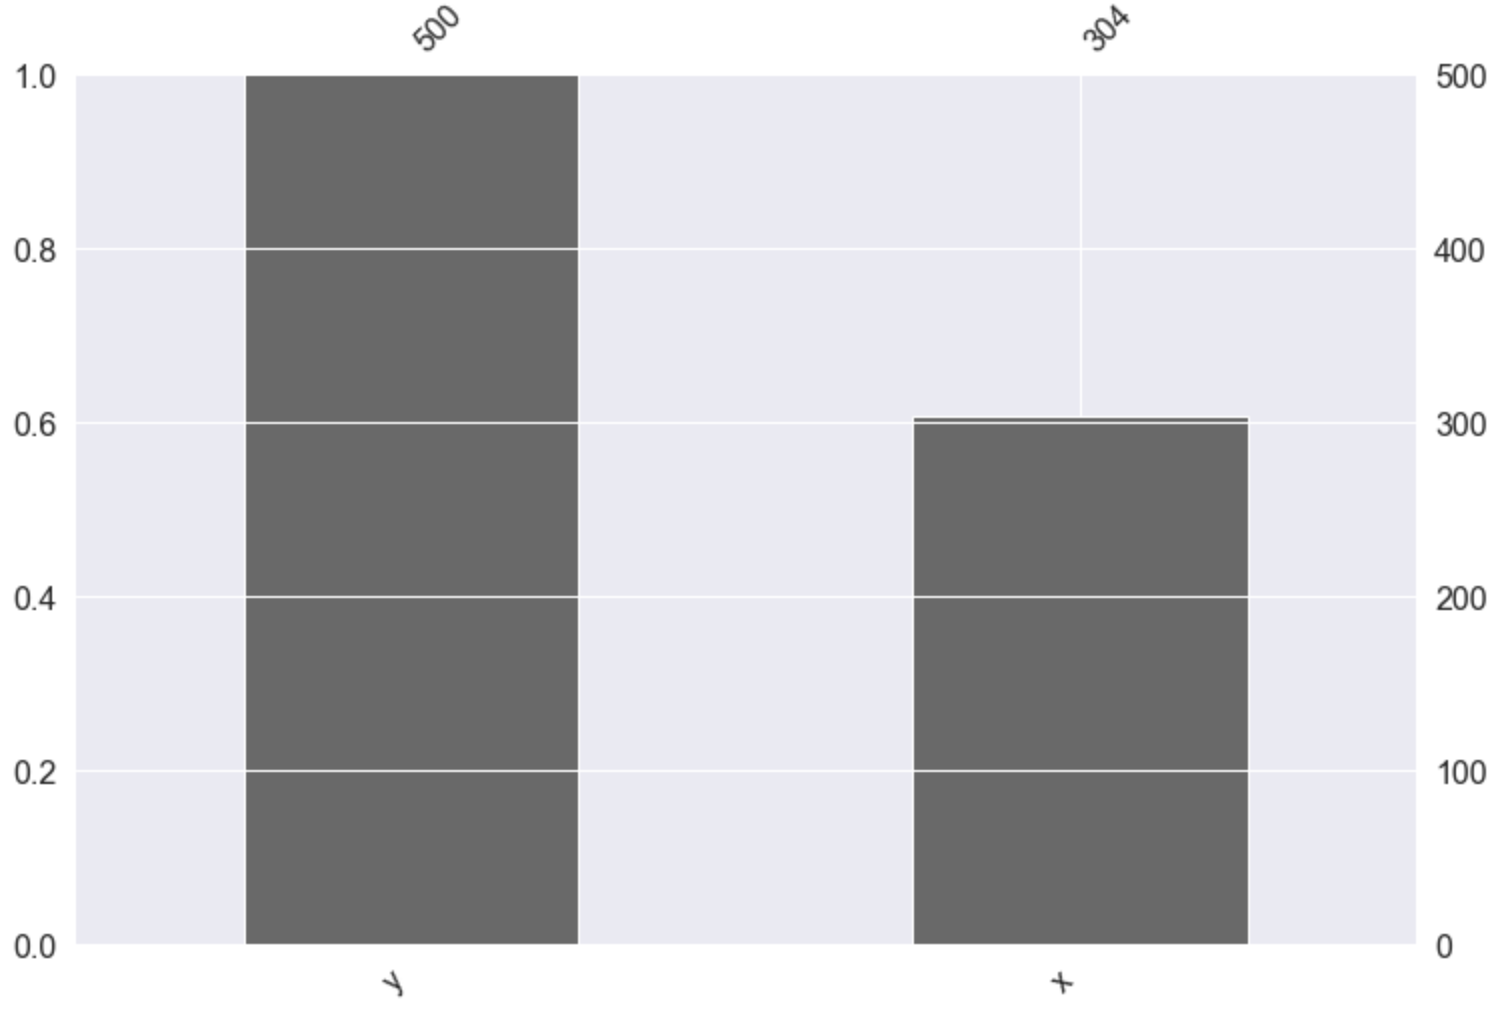
\includegraphics[width=400px]{figure/x-mis-forty-bar-mar} 

}

\caption{Missingness Percentage}\label{fig:x-mis-forty-bar-mar}
\end{figure}
---------- SWARM PLOTS HERE TOO ? --------------

\section*{Analysis Models on each
Example}\label{analysis-models-on-each-example}
\addcontentsline{toc}{section}{Analysis Models on each Example}

The sections above take the user through the data exploration phase and
multiple imputation phase of \texttt{Autoimpute}. At each step, the
authors use visualization methods from the \texttt{Autoimpute} package
to demonstrate what each imputation method does under the hood when used
in the multiple imputation framework. The next section,
\protect\hyperlink{findings}{Findings}, demonstrates how each imputation
algorithm affects the inference derived from linear regression. Results
from analysis on imputed datasets are compared to the results from
analysis on the complete dataset.

\hypertarget{findings}{\chapter*{Findings}\label{findings}}
\addcontentsline{toc}{chapter}{Findings}

\section*{Full Model Recap}\label{full-model-recap}
\addcontentsline{toc}{section}{Full Model Recap}

We begin this section with a recap of linear regression on the full
dataset. The results below serve as the benchmark for comparison. They
are considered the golden standard.

The results for the full model are displayed again:
\begin{figure}

{\centering 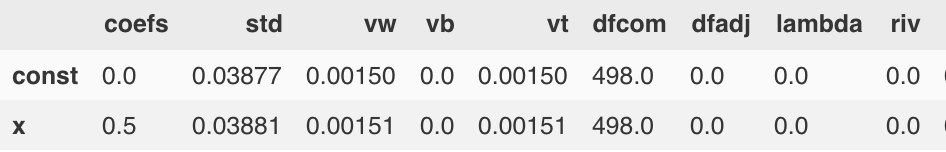
\includegraphics[width=400px]{figure/full-regression} 

}

\caption{Linear Regression Recap: Full}\label{fig:full-regression-again}
\end{figure}
Next, the authors examine how each missing data method performs and if
the imputations it generates distort the results from linear regression.
If coefficients are biased, then the imputation model used does not
produce plausible imputations that respect the original structure of the
complete data. Further, if variance measures are too narrow, then the
imputation model did not create sufficient variability to account for
uncertainty introduced by missingness, and the statistical significance
of the coefficients may be called into question.

The authors display the results of linear regression for each example in
the methodology section.

\section*{Results from Example 1}\label{results-from-example-1}
\addcontentsline{toc}{section}{Results from Example 1}

The authors review the results from a linear regression on the imputed
dataset from Example 1. Recall that Example 1 contains 40\% missingness
in the response \(y\), and the missingness mechanism is MCAR.

First, listwise delete:
\begin{figure}

{\centering 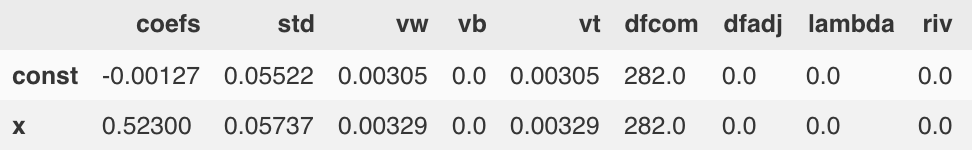
\includegraphics[width=400px]{figure/mcar-listwise-delete} 

}

\caption{Linear Regression Results under MCAR: Listwise Delete}\label{fig:mcar-listwise-delete}
\end{figure}
Next, mean imputation:
\begin{figure}

{\centering 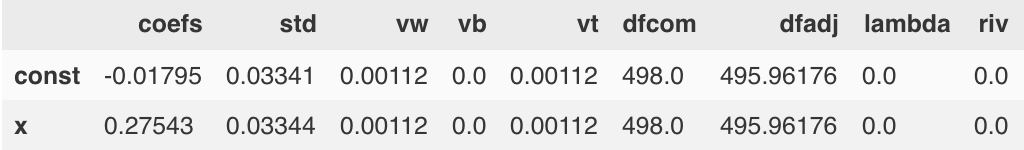
\includegraphics[width=400px]{figure/mcar-mean} 

}

\caption{Linear Regression Results under MCAR: Mean Imputation}\label{fig:mcar-mean}
\end{figure}
Next, least squares imputation:
\begin{figure}

{\centering 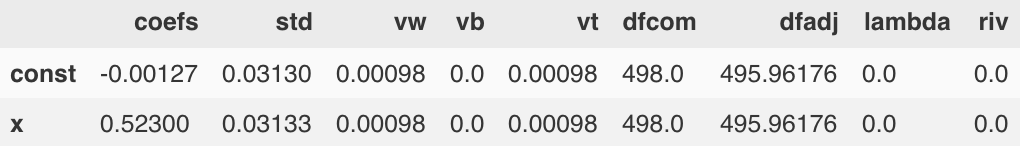
\includegraphics[width=400px]{figure/mcar-ls} 

}

\caption{Linear Regression Results under MCAR: Least Squares Imputation}\label{fig:mcar-ls}
\end{figure}
Finally, pmm imputation:
\begin{figure}

{\centering 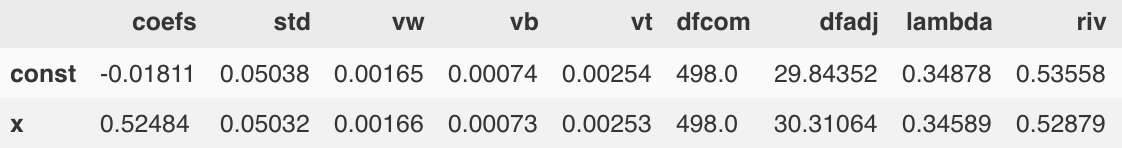
\includegraphics[width=400px]{figure/mcar-pmm} 

}

\caption{Linear Regression Results under MCAR: PMM Imputation}\label{fig:mcar-pmm}
\end{figure}
\section*{Findings from Example 1}\label{findings-from-example-1}
\addcontentsline{toc}{section}{Findings from Example 1}

The authors explore the impact each missing data method has on the
coefficient estimate for \(x\) and the resulting standard error and
variance of \(x\).

First, the authors discuss coefficient estimates. Mean imputation
produces a grossly biased parameter estimate for \(x\). This result
occurs because mean imputation thins the distribution of the variable it
imputes. As a result, mean imputation shrinks the correlation between
any feature and the imputed variable (van Buuren, ch.~1.3.1). Therefore,
the mean imputation is suboptimal. Next, note that listwise deletion,
least squares, and pmm all produce parameter estimates close to the true
value of the parameter estimate from the regression model on the
complete dataset. PMM's estimate is the least biased of the three. These
results are also expected. Under MCAR with missingness in the response
only, listwise deletion, least squares, and pmm all produce unbiased
estimates for the parameter of interest (Van Buuren, ch.~1.3.8; ch 3.4).

Next, the authors examine the impact of imputation methods on the
variance of parameter estimates. Listwise deletion produces larger
variance and standard error because the sample size used for the
regression model is reduced. Mean imputation produces similar standard
error and variance as the full regression model, because mean imputation
does not produce any variability between imputations. Results from least
squares are even worse. The standard error and variance of coefficient
estimates shrink significantly. This phenomenon stems from the fact that
least squares imputation increases the correlation between features and
the imputed variable. As a result, the variability of the imputed data
is understated, and the resulting standard error of the coefficient
estimate is far too low. This underestimation makes the coefficient seem
more statistically significant than it may be. PMM imputation, on the
other hand, increases the variance and standard error of the coefficient
estimates. It does so for a different reason than listwise deletion,
however. Notice that PMM is the only method with a non-zero value for
the variance-between. This stems from the fact that PMM produces
different parameter estimates in each analysis model applied to the
multiply imputed datasets. Therefore, when the coefficients are pooled,
additional variance results. This additional variance accurately
captures the uncertainty introduced from imputing missing values.

\section*{Results from Example 2}\label{results-from-example-2}
\addcontentsline{toc}{section}{Results from Example 2}

Next, we examine the results from a linear regression on the imputed
dataset from Example 2. Recall that Example 2 contains 40\% missingness
in the predictor \(x\), and the missingness mechanism is MAR.

First, listwise delete:
\begin{figure}

{\centering 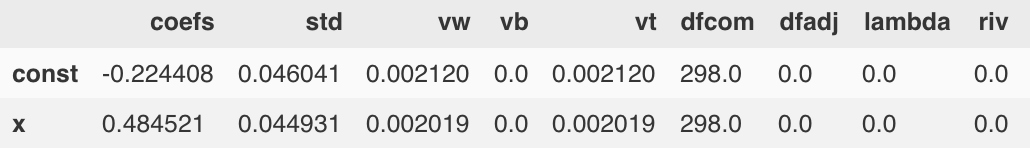
\includegraphics[width=400px]{figure/mar-listwise-delete} 

}

\caption{Linear Regression Results under MAR: Listwise Delete}\label{fig:mar-listwise-delete}
\end{figure}
Next, mean imputation:
\begin{figure}

{\centering 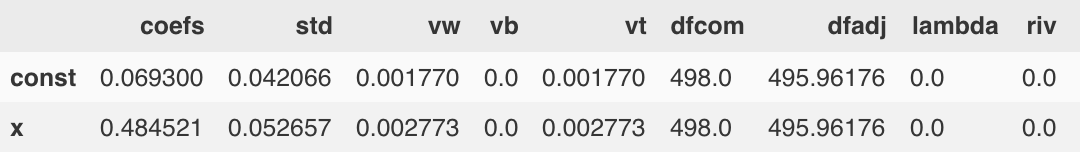
\includegraphics[width=400px]{figure/mar-mean} 

}

\caption{Linear Regression Results under MAR: Mean Imputation}\label{fig:mar-mean}
\end{figure}
Next, least squares imputation:
\begin{figure}

{\centering 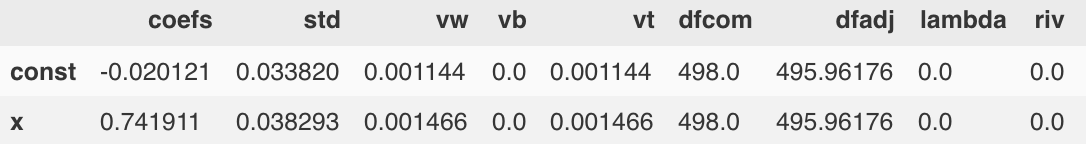
\includegraphics[width=400px]{figure/mar-ls} 

}

\caption{Linear Regression Results under MAR: Least Squares Imputation}\label{fig:mar-ls}
\end{figure}
Finally, pmm imputation:
\begin{figure}

{\centering 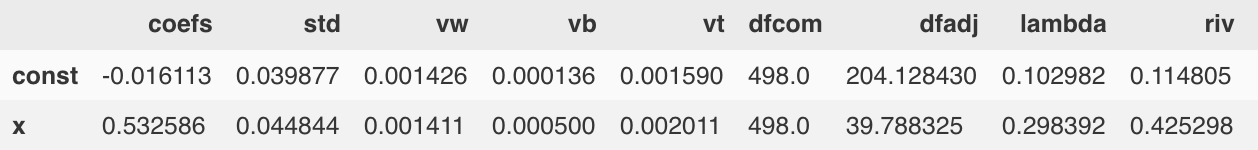
\includegraphics[width=400px]{figure/mar-pmm} 

}

\caption{Linear Regression Results under MAR: PMM Imputation}\label{fig:mar-pmm}
\end{figure}
\section*{Findings from Example 2}\label{findings-from-example-2}
\addcontentsline{toc}{section}{Findings from Example 2}

In example 2, the missing data mechanism is MAR and right-tailed.
Therefore, the probability of missingness in \(x\) increases with larger
values of \(y\). As a result, the analysis models from listwise deletion
and mean imputation are negatively biased. Least squares regression, on
the other hand, produces a coefficient that is grossly overbiased. PMM
is the only method that produces an unbiased estimate for the
coefficient.

The analysis of variance is similar to example 1. In general, listwise
deletion always enlarges the coefficient variance and standard error
because the sample size is reduced. Mean imputation ignores any
variability between imputations, and least squares inflates correlation
between features, thus deflating the standard error and variance of a
parameter estimate. PMM is the only method that retains the variability
introduced from multiple imputation, and thus it increases standard
error to account for the underlying uncertainty in the true value of
missing data points.

\section*{Inference from Examples}\label{inference-from-examples}
\addcontentsline{toc}{section}{Inference from Examples}

Whenever a researcher fits a supervised machine learning model of
imputed data, he or she should be concerned with potential bias of the
coefficient estimates and possible understatement or coefficient
standard error. The examples above show that bias and standard error are
the direct result of how imputation methods respond to the nature of
missing data and if they handle the missing data mechanism correctly.

The researcher should always select the method that produces the best
results from the analysis model. The best results stem from an
imputation method that preserves the covariance structure of the
underlying data. Therefore, in Example 2, the researcher should feel
comfortable selecting PMM as the best missing data method to use. In the
case where numerous imputation methods lead to unbiased parameter
estimates and sufficient standard error for coefficients, the researcher
must then consider other factors related to the underlying missing data
method. In the MCAR example, both PMM and listwise deletion do a good
job. But PMM is computationally expensive, and the results from PMM vary
each time the researcher imputes the data (assuming no seed is set). In
this case, listwise deletion may actually be prefered.

These examples demonstrate that there is no free lunch when it comes to
analysis of imputed data. The researcher must consider multiple
imputation models and assess how they affect bias and variance of
coefficients. Additionally, the researcher must consider the
computational cost of the underlying imputation algorithm and its
flexibility to extend to other scenarios with missing data. Some
imputation methods can always be rejected, such as mean and least
squares imputation. Other methods, however, must be vetted and selected
with careful consideration.

\chapter*{Conclusion}\label{conclusion}
\addcontentsline{toc}{chapter}{Conclusion}

In summary, this project demonstrates how complex it is to hanlde
missing data. The authors provide an end-to-end methodology to explore
missing data, handling it using missing data methods, and analyze the
impact of missing data methods on supervised analysis models. At the
beginning of this text, the researchers proposed four key objectives:
describe and visualize the extent of the missing value problem; examine
factors related to missingness; develop methods to impute missing data;
and measure the impact of imputation on inference derived from
supervised learning. Throughout this text, the researchers addressed
each objective. To address each objective, the researchers used
Autoimpute - the open-source Python package the authors created for
users grappling with missing data. The Autoimpute package provides
methods to explore missingness, implement imputation methods, and
analyze their impact on analytical models in a flexible way.

This report focuses on establishing a solid foundation around the
concepts missing data and imputation and demonstrates examples of
missing data analysis on different types of missing data. Ultimately,
this research provides Python-savy data practitioners a framework to use
to explore missingness in their datasets, perform imputation methods,
and assess the impact of imputation on analytical models downstream.
Hopefully, users of the Autoimpute package are now well equipped to deal
with missing data if and when it arises during their own machine
learning research.

\chapter*{Recommendations}\label{recommendations}
\addcontentsline{toc}{chapter}{Recommendations}

This research explores missingness and outlines a framework through
which a data practitioner can conduct missing data and imputation
analysis. The researchers recommend data practitioners use the
flexibility, simplicity, and granularity of the Autoimpute package to
conduct their own missing data analyses. To start, data practitioners
should review the Autoimpute tutorials website to get a better
understanding of how the package works and how and end user can get the
most out of its functionality. source code, either locally after a
\texttt{pip\ install} or directly on Autoimpute's github page. Once
familiar with the package, data practitioners should
\texttt{pip\ install} the publicly available package from GitHub, review
the source code, and start using the package in their own analysis. If
challenges arise when using the package, researchers should contact the
authors, preferably by submitting a bug report, feature request, or pull
request depending on the nature of the issue. Lastly, the researchers
hope end users share feedback about the Autoimpute package with the
authors and share any interesting results found in personal analyses.

\appendix

\chapter{Autoimpute References}\label{autoimpute-references}

\texttt{Autoimpute} is an open-source Python package distributed under
the MIT license. The package is hosted on github and registered with the
official Python Package Index. The authors also host a website that
explores Autoimpute in more detail and provides in-depth tutorials on
how end-users can get the most out of the package. The table below
provides links to the package and the author's website.
\begin{table}[!h]

\caption{\label{tab:appendixa}Autoimpute Sources}
\begin{tabu} to \linewidth {>{\raggedright\arraybackslash}p{5em}>{\raggedright}X}
\toprule
\begingroup\fontsize{13}{15}\selectfont \textbf{Source}\endgroup & \begingroup\fontsize{13}{15}\selectfont \textbf{Link}\endgroup\\
\midrule
Github & https://github.com/kearnz/autoimpute\\
PyPI & https://pypi.org/project/autoimpute/\\
Website & https://kearnz.github.io/autoimpute-tutorials/\\
\bottomrule
\end{tabu}
\end{table}
\chapter{Missingness Notation
Cheatsheet}\label{missingness-notation-cheatsheet}
\begin{longtabu} to \linewidth {>{\raggedright\arraybackslash}p{5em}>{\raggedright}X}
\caption{\label{tab:appendixbnotation}Notation}\\
\toprule
\begingroup\fontsize{13}{15}\selectfont \textbf{Notation}\endgroup & \begingroup\fontsize{13}{15}\selectfont \textbf{Description}\endgroup\\
\midrule
$n$ & The number of records or observations in a matrix\\
$p$ & The number of columns or features in a matrix\\
$Y$ & The complete data matrix of observed and missing records\\
$Y_{obs}$ & Records within $Y$ that are completely observed for all columns $p$\\
$Y_{mis}$ & Records within $Y$ with a missing value in any column in $p$\\
\addlinespace
$y_{ij}$ & A scalar value $y$ in row $i$ and column $j$ of matrix $Y$\\
$R$ & The missing indicator matrix, where each value $r_{ij} \in 0,1$\\
$r_{ij}$ & A scalar value $r$ in row $i$ and column $j$ of matrix $R$\\
$\psi$ & The parameters of the missing data model\\
$m$ & The number of complete datasets $Y$ to impute independently\\
\addlinespace
$I_j$ & The influx coefficient\\
$O_j$ & The outflux coefficient\\
$Q$ & The population parameter of scientific interest\\
$\hat Q$ & The estimate for $Q$ using hypothetically complete data\\
$U$ & The variance-covariance matrix of estimate $\hat Q$\\
\addlinespace
$\bar Q$ & The pooled parameter estimate of $Q$ under multiple imputation\\
$\bar U$ & The variance-within under multiple imputation\\
$B$ & The variance-between under multiple imputation\\
$T$ & The total variance under multiple imputation\\
\bottomrule
\end{longtabu}
\chapter{Missingess Expression
Cheatsheet}\label{missingess-expression-cheatsheet}
\begin{longtabu} to \linewidth {>{\raggedright}X>{\raggedright}X}
\caption{\label{tab:appendixcexpressions}Expressions}\\
\toprule
\begingroup\fontsize{13}{15}\selectfont \textbf{Expression}\endgroup & \begingroup\fontsize{13}{15}\selectfont \textbf{Description}\endgroup\\
\midrule
$Y = (Y_{mis}, Y_{obs})$ & The complete data matrix equals the conjoined $Y_{obs}$ and $Y_{mis}$\\
$r_{ij} = 0$ & When a value $r_{ij}=0$, the corresponding value $y_{ij}$ is missing\\
$r_{ij} = 1$ & When a value $r_{ij}=1$, the corresponding value $y_{ij}$ is observed\\
$P(R\mid Y_{obs}, Y_{mis},\psi)$ & General expression for a missing data model. Also form for MNAR\\
$P(R=0\mid Y_{obs},Y_{mis},\psi) = P(R=0\mid \psi)$ & Reducible form of the missing data model under MCAR\\
\addlinespace
$P(R=0\mid Y_{obs},Y_{mis},\psi) = P(R=0\mid Y_{obs}, \psi)$ & Reducible form of the missing data model under MAR\\
$P(Y_{mis}\mid Y_{obs}, R)$ & General expression for an imputation model\\
$P(Y\mid Y_{obs}, R=1) = P(Y\mid Y_{obs}, R=0)$ & Implication of ignorability in which imputation models can safely ignore $\psi$\\
$I_j = \frac{\sum_j^p\sum_k^p\sum_i^n (1-r_{ij})r_{ik}}{\sum_k^p\sum_i^n r_{ik}}$ & The forumla for influx coefficient\\
$O_j = \frac{\sum_j^p\sum_k^p\sum_i^n r_{ij}(1-r_{ik})}{\sum_k^p\sum_i^n 1-r_{ij}}$ & The formula for outflux coefficient\\
\addlinespace
$E(\hat Q|Y) = Q$ & The equality necessary for unbiasedness of an estimate $\hat Q$ conditional on $Y$\\
$\bar Q = \frac{1}{m}\sum_{\ell=1}^m \hat Q_\ell$ & The pooled estimate for $Q$ is the mean of $m$ $\hat Q$ estimates from $m$ imputations\\
$\bar U = \frac{1}{m}\sum_{\ell=1}^m \bar U_\ell$ & The variance within is the mean of the $m$ $\hat U$ estimates from $m$ imputations\\
$B = \frac{1}{m-1}\sum_{\ell=1}^m (\hat Q_\ell-\bar Q)(\hat Q_\ell-\bar Q)'$ & The variance between is the additional variance in estimating $\hat Q$ during $m$ imputations\\
$T = \bar U + B + \frac{B}{m}$ & The total variance is the sum of variance within, variance between, and added variance from finite number of imputations $m$\\
\bottomrule
\end{longtabu}
\chapter{Concepts Related to
Missingness}\label{concepts-related-to-missingness}
\begin{longtabu} to \linewidth {>{\raggedright\arraybackslash}p{7em}>{\raggedright}X}
\caption{\label{tab:appendixdconcepts}Concepts}\\
\toprule
\begingroup\fontsize{13}{15}\selectfont \textbf{Concept}\endgroup & \begingroup\fontsize{13}{15}\selectfont \textbf{Definition}\endgroup\\
\midrule
complete data matrix & The complete matrix $Y$, which is comprised of $Y_{obs}$ and $Y_{mis}$\\
missing indicator matrix & Missing indicator $R$ suggests which values in $Y$ are missing\\
missing data mechanism & Process that governs relationship b/w observed and $P(missing)$\\
missing data model & Formalizes relationship specified by missing data mechanism\\
MCAR & Missing data mechanism depends on $\psi$ only\\
\addlinespace
MAR & Missing data mechanism depends on $Y_{obs}$ and $\psi$ only\\
MNAR & Missing data mechanism depends on $Y_{obs}$, $Y_{mis}$, and $\psi$\\
ignorability & Criteria required for imputation models to ignore $\psi$\\
missing data pattern & Various ways in which data can be missing throughout a dataset\\
missing data method & Method used to handle missing data. Use deletion or imputation\\
\addlinespace
deletion & Discard missing values from the dataset\\
imputation model & Replace missing values with imputations from imputation model\\
analysis model & A supervised machine learning model applied to imputed data\\
target & Column with missing values to be imputed\\
univariate & Models using target to determine imputation for target\\
\addlinespace
multivariate & Models using features to predict imputed values for target\\
missing data pattern & Pattern suggesting information transferrable b/w variables\\
single imputation & Impute missing values once prior to analysis\\
multiple imputation & Impute missing values $m$ times prior to analysis\\
influx & Candidates to be imputed using the other predictors\\
\addlinespace
outflux & Variables useful as predictors to impute a target variable\\
pooled parameter estimate & The coefficients of an analysis model under multiple imputation\\
variance within & The average of the variance of the parameter estimate from each imputation\\
variance between & The variance introduced from different parameter estimates across imputations\\
total variance & The accurate representation of variance under multiple imputation\\
\bottomrule
\end{longtabu}
\chapter{Univariate Imputation
Methods}\label{univariate-imputation-methods}
\begin{longtabu} to \linewidth {>{\raggedright\arraybackslash}p{7em}>{\raggedright}X}
\caption{\label{tab:appendixeunivar}Univariate Methods}\\
\toprule
\begingroup\fontsize{13}{15}\selectfont \textbf{Method}\endgroup & \begingroup\fontsize{13}{15}\selectfont \textbf{Description}\endgroup\\
\midrule
mean & Mean imputation finds the mean of observed values in target variable $y$. It then imputes any missing values in $y$ with the observed mean.\\
median & Median imputation finds the median of observed values in target variable $y$. It then imputes any missing values in $y$ with the observed median.\\
mode & Mode imputation finds the mode of observed values in target variable $y$. It then imputes any missing values in $y$ with the observed mode. If multiple modes exist, Autoimpute gives users the option to take the first mode, the last mode, or randomly sample the modes when imputing missing values.\\
random & Random imputation imputes each missing value in target $y$ by randomly sampling from the observed values in $y$.\\
norm & Norm imputation constructs a normal distribution parameterized by the mean and variance of the observed values in target $y$. Missing values are then imputed with random draws from the constructed normal distribution.\\
\addlinespace
categorical & Categorical imputation constructs a discrete categorical distribution parameterized by the proportions of each distinct label in target $y$. Missing values are then imputed with draws from the constructed categorical distribution, where the probability of a given label being drawn depends on its proportion within the categorical distribution.\\
interpolation & Interpolation imputation constructs new data points within the range of a discrete set of known data points. Autoimpute supports linear, quadratic, cubic, polynomial, and spline interpolation.\\
last observation carried forward (LOCF) & LOCF imputes missing values by carrying forward the last observed value. Therefore, the method respects the order of the records in target $y$.\\
next observation carried backward (NOCB) & NOCB imputes missing values by carrying backward the next observed value. Therefore, the method respects the order of the records in target $y$.\\
\bottomrule
\end{longtabu}
\chapter{Multivariate Imputation
Methods}\label{multivariate-imputation-methods}
\begin{longtabu} to \linewidth {>{\raggedright\arraybackslash}p{7em}>{\raggedright}X}
\caption{\label{tab:appendixfmultivar}Multivariate Methods}\\
\toprule
\begingroup\fontsize{13}{15}\selectfont \textbf{Method}\endgroup & \begingroup\fontsize{13}{15}\selectfont \textbf{Description}\endgroup\\
\midrule
linear regression & Linear Regression imputation fits a linear model on observed data, where $y$ is the target variable to be imputed and $X$ is the design matrix. The model then finds the records in $X$ where $y$ is missing. These records in $X$ are used to generate predictions from the linear model. Those predictions become the imputations for missing values in $y$\\
binomial logistic regression & Binary Logistic Regression imputation fits a binary logistic model on observed data, where $y$ is the target variable to be imputed and $X$ is the design matrix. The model then finds the records in $X$ where $y$ is missing. These records in $X$ are used to generate predictions from the binary logistic model. Those predictions become the imputations for missing values in $y$\\
multinomial logistic regression & Multinomial Logistic Regression imputation fits a multinomial logistic model on observed data, where $y$ is the target variable to be imputed and $X$ is the design matrix. The model then finds the records in $X$ where $y$ is missing. These records in $X$ are used to generate predictions from the multinomial logistic model. Those predictions become the imputations for missing values in $y$\\
stochastic regression & Stochastic Regression imputation fits a linear model on observed data, where $y$ is the target variable to be imputed and $X$ is the design matrix. The algorithm then stores a normal distribution for the errors from the fit linear model. The model then finds the records in $X$ where $y$ is missing. These records in $X$ are used to generate predictions from the linear model. For each prediction, the algorithm adds a random draw from the distribution of errors. Those predictions + random draws become the imputations for missing values in $y$\\
bayesian linear regression & Bayesian linear regression imputation imputes missing values using random draws from the posterior predictive distribution of the missing data $Y_{mis}$. These draws take into account the posterior distribution of the linear model parameters, which in this case are $\hat{\beta}$ coefficients.\\
\addlinespace
bayesian binary logistic regression & Bayesian binary logistic regression imputation imputes missing values using random draws from the posterior predictive distribution of the missing data $Y_{mis}$. These draws take into account the posterior distribution of the binary logistic model parameters, which in this care are the probabilities of class membership.\\
predictive mean matching (PMM) & PMM imputation is a multi-step procedure. First, a linear model is fit on the observed data for target $y$ and $X$ to obtain $\hat{\beta}$ coefficients. Then, a bayesian model is fit, and the algorithm produces a new set of $\dot{\beta}$ coefficients using random draws from the posterior predictive distribution of $\hat{\beta}$. The coefficients $\hat{\beta}$ are used to make predictions for observed $y$, while $\dot{\beta}$ are used to make predictions for missing $y$. For each case where $y$ is missing, the algorithm finds the closest $n$ predicted values among cases where $y$ is observed. The algorithm then randomly samples the $n$ closest predictions, selecting one, and eventually imputes the missing data with the truly observed value of $y$. The standard distance used to measure 'closeness' is manhattan distance. $n$ represents the number of neighbors to find, which generally defaults to 5.\\
local residual draws (LRD) & LRD imputation begins by replicating the process for PMM. Once the truly observed value of $y$ is selected through the PMM process, LRD adds the distance to that value. The missing value is then imputed using the sum of the observed value of $y$ and the distance.\\
\bottomrule
\end{longtabu}
\backmatter

\chapter*{References}\label{references}
\addcontentsline{toc}{chapter}{References}

\markboth{References}{References}

\noindent

\setlength{\parindent}{-0.20in} \setlength{\leftskip}{0.20in}
\setlength{\parskip}{8pt}

\hypertarget{refs}{}
\hypertarget{ref-allison_handling_2012}{}
Allison, P. (2012). Handling missing data by maximum likelihood.
\emph{SAS Global Forum 2012}. Haverford; PA; USA: Statistical Horizons.
Retrieved from
\url{https://statisticalhorizons.com/wp-content/uploads/MissingDataByML.pdf}

\hypertarget{ref-allison_handling_2014}{}
Allison, P. (2014, June 13). Listwise deletion: It's not evil. Retrieved
from
\url{https://statisticalhorizons.com/listwise-deletion-its-not-evil}

\hypertarget{ref-bilogur_missingno_2018}{}
Bilogur, A. (2018). Missingno: A missing data visualization suite.
\emph{The Journal of Open Source Software}, \emph{3}(22), 547.
\url{http://doi.org/10.21105/joss.00547}

\hypertarget{ref-econ_commission}{}
COMMISSION, U. N. S., \& EUROPE, E. C. F. (2000). GLOSSARY OF TERMS ON
STATISTICAL DATA EDITING. Geneva. Retrieved from
\url{https://ec.europa.eu/eurostat/ramon/statmanuals/files/UN_editing_glossary_2000.pdf}

\hypertarget{ref-peng_dong}{}
Dong, Y., \& Peng, C.-Y. J. (2013). Principled missing data methods for
researchers. \emph{SpringerPlus}, \emph{2}(1).
\url{http://doi.org/10.1186/2193-1801-2-222}

\hypertarget{ref-gelman_data_2017}{}
Gelman, A., \& Hill, J. (2017). \emph{Data Analysis using Regression and
Multilevel/Hierarchical Models}. Cambridge ; New York: Cambridge
University Press.

\hypertarget{ref-lu_robust_2014}{}
Lu, Z. (., \& Zhang, Z. (2014). Robust growth mixture models with
non-ignorable missingness: Models, estimation, selection, and
application. \emph{Computational Statistics \& Data Analysis},
\emph{71}, 220--240. \url{http://doi.org/10.1016/j.csda.2013.07.036}

\hypertarget{ref-morris_tuning_2014}{}
Morris, T. P., White, I. R., \& Royston, P. (2014). Tuning multiple
imputation by predictive mean matching and local residual draws.
\emph{BMC Medical Research Methodology}, \emph{14}(1).
\url{http://doi.org/10.1186/1471-2288-14-75}

\hypertarget{ref-introduction_to_sas_notitle_2017}{}
MULTIPLE IMPUTATION IN STATA. (2017). \emph{UCLA: Institute for Digital
Research \& Education}. Retrieved from
\url{https://stats.idre.ucla.edu/stata/seminars/mi_in_stata_pt1_new/}

\hypertarget{ref-nakagawa_chapter_2015}{}
Nakagawa, S. (2015). \emph{CHAPTER 4 Missing data : Mechanisms , methods
, and messages}.

\hypertarget{ref-rubin_inference_1976}{}
Rubin, D. B. (1976). Inference and missing data. \emph{Biometrika},
\emph{63}(3), 581--592. \url{http://doi.org/10.1093/biomet/63.3.581}

\hypertarget{ref-schouten_generating_2018}{}
Schouten, R. M., Lugtig, P., \& Vink, G. (2018). Generating missing
values for simulation purposes: A multivariate amputation procedure.
\emph{Journal of Statistical Computation and Simulation}, \emph{88}(15),
2909--2930. \url{http://doi.org/10.1080/00949655.2018.1491577}

\hypertarget{ref-van_buuren_flexible_2018}{}
van Buuren, S. (2018). \emph{Flexible Imputation of Missing Data} (2nd
ed.). Chapman; Hall/CRC. Retrieved from
\url{https://stefvanbuuren.name/publication/2018-01-01_vanbuuuren2018/}

\hypertarget{ref-mice_package}{}
van Buuren, S., \& Groothuis-Oudshoorn, K. (2011). mice: Multivariate
imputation by chained equations in r. \emph{Journal of Statistical
Software}, \emph{45}(3), 1--67. Retrieved from
\url{https://www.jstatsoft.org/v45/i03/}

\hypertarget{ref-mass_package}{}
Venables, W. N., \& Ripley, B. D. (2002). \emph{Modern applied
statistics with s} (Fourth). New York: Springer. Retrieved from
\url{http://www.stats.ox.ac.uk/pub/MASS4}

\hypertarget{ref-vink_towards_nodate}{}
Vink, G. (n.d.). Towards a Standardized Evaluation of Multiple
Imputation Routines. Retrieved from
\url{https://www.gerkovink.com/docs/Standardized\%20evaluation.pdf}

\hypertarget{ref-xie_measuring_2018}{}
Xie, H., Gao, W., Xing, B., Heitjan, D. F., Hedeker, D., \& Yuan, C.
(2018). Measuring the impact of nonignorable missingness using the r
package isni. \emph{Computer Methods and Programs in Biomedicine},
\emph{164}, 207--220. \url{http://doi.org/10.1016/j.cmpb.2018.06.014}

\hypertarget{ref-yin_simulation_based_2015}{}
Yin, P., \& Shi, J. Q. (2015). Simulation-based sensitivity analysis for
non-ignorable missing data. \emph{arXiv:1501.05788 {[}Stat{]}}.
Retrieved from \url{http://arxiv.org/abs/1501.05788}

\hypertarget{ref-yu_comparative_2017}{}
Yu, A., Wagner, J., \& Murugesan, M. (2017). \emph{Comparative
Evaluation of Recent ML Based Missing Data Imputation Methods with
NORC's Survey of Consumer Finances} (PhD thesis). University of Chicago
Graham School.


% Index?

\end{document}
